%% USPSC-Cap2-Desenvolvimento.tex 

% ---
% Este capítulo, utilizado por diferentes exemplos do abnTeX2, ilustra o uso de
% comandos do abnTeX2 e de LaTeX.
% ---


\chapter{Development}
\label{cap:development}

\section{Definitions}
\label{sec:definitions}

\subsection{Mathematical notation}
\label{sec:notation}

For any given matrix $M$, we denote by $M\el {ij}$ its element on the $i$-th row
and $j$-th column ($i, j \in \mathbb{N}^*$). Analogously, we represent by
$M\el{i\cdot}$ the vector containing $M$'s $i$-th row so that $M\el{i\cdot}\el j
= M\el{ij}$ and by $M\el{\cdot j}$ the column vector
$((M^\intercal)\el{j\cdot})^\intercal$ referring to the $j$-th column of $M$ so
that $M\el{\cdot j}\el{i1} = M\el{ij}$. Defining the index notations as
superscripts frees the subscripts to be used only as indentifiers, naming the
matrix or vector as a whole and not in an element-wise fashion. Indices are also
always represented by a single letter, to dispense the use of separators between
them.

% If multiple characters are needed, a comma or parentheses can be used
% $X\el{25,389}$ $X\el{(25)(389)}$

Inspired by the usual notation $|\cdot|$ for the cardinality of a set, we write
the total number of $M$'s rows as $|M|_i$ and its number of columns as $|M|_j$.
The total number of elements in $M$ is written $|M| = |M|_j|M|_i$, not to be
confused with the determinant of $M$.

We display filtered matrices or vectors by writing the condition as the index,
optionally enclosed by parentheses when necessary or improving readability (Eq.
\ref{eq:filter_notation}).
%
\begin{equation*}
    M\el{(i<3)j} \equiv \{M\el{kj}\;\mid \; k < 3\}
    \label{eq:filter_notation}
\end{equation*}

When summing over all indices in a given dimension, we took the freedom of
omitting the start and end positions (\autoref{eq:sum_notation}).
%
\begin{equation*}
    \sum_i M\el{ij} \equiv \sum_{i=1}^{|M|_i} M\el{ij}
    \label{eq:sum_notation}
\end{equation*}

We also made the choice of representing averages in a more concise way,
optionally pondered by sets of $w_1$ and $w_2$ weights in each respective axis
(\autoref{eq:avg_notation}).
%
\begin{equation}
    \begin{split}
        M\mel i \el j
            &\equiv \frac{\sum_i w_1\el i M\el{ij}} {\sum_i w_1\el i}\\
        M\el i \mel j
            &\equiv \frac{\sum_j w_2\el j M\el{ij}} {\sum_j w_2\el j}\\
        M\mel{ij}
            &\equiv \frac{\sum_j \sum_i w_2\el j w_1\el i M\el{ij}} {\sum_j \sum_i w_2\el j w_i\el i}
    \end{split}
    \label{eq:avg_notation}
\end{equation}

The enclosing of indices within brackets also allows for the omission of
parentheses when concomitantly using exponents, as exemplified by Eq.
\ref{eq:avg_index_notation}, and we additionally reserve ourselves the freedom
of representing each index only once, which in the last two shown cases requires
preemptively defining that $i$ and $j$ respectively represent rows and columns.
Notice that dispensing parentheses makes important the order in which the
exponent and averaged indices (those within $\langle \cdot \rangle$) appear. The
position of indices within $[\cdot]$ is however facultative, and is here chosen
to be as close as $M$ as possible in order to avoid confusion with $M^2=MM$.
Also notice that the indices within $[\cdot]$ will be the indices of the
resulting matrix or vector.
%
\begin{equation}
    \begin{split}
        M \el {ij} ^2 &= ((M \el{ij})^2)\el{ij}\\
        M \mel {ij} ^2 &= (M \mel{ij})^2\\
        M ^2 \mel {ij} &= (M \el{ij}^2)\mel{ij}\\
        % M \el i \mel j ^2 &= ((M \el i \mel j)^2)\el i\\  % corollary
        % M \mel i \el j ^2 &= ((M \mel i \el j)^2)\el j\\  % corollary
        %
        M \el i ^2 \mel j &= M \el{ij}^2\mel j\\
        M \el j ^2 \mel i &= M \el{ij}^2\mel i
        %M \el i ^2 \mel j &= (M \el{ij}^2)\el i\mel j\\
        %M \el j ^2 \mel i &= (M \el{ij}^2)\mel i\el j\\
        %
        % M \mel i ^2 \el j &= (M \mel i \el j^2) \el j
        % M \el i \mel j ^2 &= (M \el i \mel j^2) \el i
    \end{split}
    \label{eq:avg_index_notation}
\end{equation}


\subsection{Problem statement}
\label{sec:problem_statement}

The supervised machine learning applications focus on modeling a function $f
\colon \mathbb{R}^{n_f} \to \mathbb{R}^{n_o}$ whose exact underlying mechanism
is unknown or costly to implement. As a result, the only information available
about such mapping is a set of inputs $\{x_i \in \mathbb R^n_f\}$ and their
corresponding outputs $\{y_i \in \mathbb R^n_o\}$ of that given function. The
goal is therefore to build an \textit{in silico} model (or estimator) $\tilde f$
that approximates $f$, yielding as similar as possible outputs for the same
given input, even and especially for outputs not utilized in the process of
building $\tilde f$.
%TODO: i1 i2 instead of i k.
%TODO: define 'sample' or 'instance'

%This includes a plethora of real-life phenomena, such as {...}.
% define sample/instance

The known input vectors are usually organized as rows of an $X$ matrix so that
$X\el{ij} = x_i\el j$, and we refer as \emph{feature} or \emph{attribute} to
each specific horizontal position $j$ of $x\el j$, which corresponds to a column
of $X$. Likewise, a $Y$ matrix is built with their corresponding outputs
($Y\el{ik} = y_i\el k$). Commonly referred to as "targets" in the context of
regression learning, we here call the known outputs of the modeled process by
\emph{labels}, as in classification, even if real-valued, to avoid confusion
when referring to the protein targets of a drug.

In the present setting, we concentrate on problems involving the interaction of
two domains of instances (also called sample groups). As such, each sample
domain forms a different $X$ matrix, that we term $X_1$ and $X_2$. Only
inter-domain interactions are allowed, that is, instances are restricted from
interacting with others in the same sample group, so that the interaction
network constitutes an undirected bipartite graph.

The output, in our case, is any scalar piece of information describing the
interaction between a given instance pair, such as the rating of a movie given
by a user or a kinetic parameter of an enzyme-substrate reaction. The labels are
then disposed in a $|X_1|_i$ by $|X_2|_i$ adjacency matrix $Y$ (also called
interaction matrix) so that the function to be modeled can now be formulated as
mapping the pair's vector representations to the interaction label $f\colon
(X_1\el{i\cdot},\; X_2\el{k\cdot}) \mapsto Y\el{ik}$.

Since each sample in $X_1$ refers to a \emph{row} of $Y$ and each sample in
$X_2$ corresponds to a \emph{column} of $Y$, we sometimes refer to the sample
domains of $X_1$ and $X_2$ as \emph{row samples} and \emph{column samples},
respectively. We call these datasets \emph{bipartite}, to differentiate from the
more common \emph{monopartite} problems, in which a single $X$ matrix is
utilized.
%TODO monopartite?

%PU data, binary, drug-target

%Train test

% Let $X_a$ be a feature matrix, the index $a$ representing each the two
% bipartite sets of instances, such that each instance is written $X_a \el i\;
% \forall\; i \in \mathbb N,\, 1 \le i \le |X_a|_i$ and each instance's feature
% is denoted $X_a\el{i, j} \;\forall\; j \in \mathbb N,\, 1 \le j \le |X_a|_j$.
% Since data is bipartite in the setting we are considering, $a$ can only assume
% the values $1$ or $2$.

% Let $Y$ be the $(n_{1s}, n_{2s})$ labels matrix such that the element $Y\el{i,
% j}$ characterizes the interaction occurring between the instances $X_1\el i$
% and $X_2\el j$.

% $X$ in algorithms is $X_\text{SGSO}$ or ... all info about X
\section{Datasets}
\label{sec:datasets}

We gathered ten publicly available interaction datasets to evaluate the performance of the proposed models. Quantitative information about the datasets is presented in table 2%\ref{main:tab:datasets}%
, and more detailed descriptions are provided below.

%\subsection{DPI-E, DPI-G, DPI-I, DPI-N~\cite{yamanishi2008}}
%\subsection{DPI-E, DPI-G, DPI-I, DPI-N}

These datasets comprise drug-protein interactions for four distinct classes of proteins: enzymes, GPCRs, ion channels, and nuclear receptors, respectively. Drug similarities were computed using the SIMCOMP metric, while protein similarities were computed as normalized scores of Smith-Waterman pairwise alignments~\cite{yamanishi2008}.

%\subsection{ERN~\cite{faith2007} and SRN~\cite{macisaac2006, hughes2000, hu2007, chua2006, schrynemackers2015}}
The datasets represent interactions between genes and transcription factors in \textit{E. coli} and \textit{S. cerevisiae}, respectively. Gene and TF features are initially composed of experimentally measured expression levels and, in SRN, gene motif features~\cite{brohee2011,schrynemackers2015}. We compute the RBF kernel of such values to obtain the final similarity matrices. %TODO rbf equation or cite

%\subsection{DAVIS~\cite{davis2011,pahikkala2015}}
The DAVIS dataset contains experimentally measured drug-kinase dissociation constants~\cite{davis2011}. The dataset was binarized by considering interactions with dissociation constants $\le 30 nM$ as the positive ones, as suggested by \cite{pahikkala2015}. Drug similarities were computed using the Extended Connectivity Fingerprints (ECFP4)~\cite{rogers2005, pahikkala2015} while protein similarities were taken as the normalized Smith-Waterman score~\cite{yamanishi2008,pahikkala2015}.

%\subsection{KIBA~\cite{tang2014,he2017simboost,huang2020deeppurpose}}
The KIBA dataset was initially built by \citeauthor{tang2014} and contains experimentally verified affinity scores between kinase and kinase inhibitors.

\cite{he2017simboost} further processed the dataset by removing all drugs and targets with less than 10 observations. In alignment with \cite{tang2014,he2017simboost}, we consider positive interactions as those with $log_10$ KIBA-scores $\leq 3.0$ to reframe the task as binary classification.

The utilized version of the dataset with corresponding amino acid sequences and SMILES representations were provided by \cite{huang2020deeppurpose}. From them, we generated the protein similarity matrix using the same procedure employed in the preprocessing of NPInter proteins. The drug similarities were computed similarly to how \cite{pahikkala2015} processed the DAVIS dataset, using the Tanimoto distances of ECFP4 fingerprints~\cite{rogers2005, pahikkala2015}. The Python library \texttt{rdkit}~\cite{rdkit} was used to this calculation.


%\subsection{mirTarBase~\cite{hsu2011mirtarbase, huang2022mirtarbase}}
The mirTarBase dataset contains experimentally validated microRNA-messengerRNA interactions. MicroRNA sequences were obtained from miRBase~\cite{griffiths2006mirbase} while transcript sequences were obtained from GENCODE~\cite{frankish2021gencode}. The longest transcript for each gene was selected and the 3' UTR exonic sequences were recovered from the genome and annotation files provided by GENCODE. The similarity matrices were then built from the normalized Smith-Waterman~\cite{yamanishi2008} alignment scores among microRNAs and among the genes' 3' UTRs. The alignments were performed using the BLASTN substitution matrix and no gap penalty, with the help of the Biopython package~\cite{cock2009biopython}.

Each miRNA was required to have at least 10 interactions in the dataset, and each gene was required to have at least 100 interactions.

%\subsection{NPInter~\cite{wu2006npinter, teng2020npinter}}
Interactions between long non-coding RNAs (lncRNA) and proteins were recovered from NPInter~\cite{wu2006npinter, teng2020npinter}. The lncRNA sequences were obtained from NONCODE~\cite{zhao2016noncode} and the protein sequences were obtained from UniProt~\cite{uniprot2019}. The similarity matrices were built from the normalized Smith-Waterman~\cite{yamanishi2008} alignment scores among lncRNAs and among the proteins. Similarly to the preprocessing of mirTarBase, we leveraged the Biopython package~\cite{cock2009biopython} to perform the alignments. using the BLASTN and BLOSUM62 substitution matrices for the lncRNA and protein alignments, respectively, and no gap penalty in both cases.

Each lncRNA was required to interact with 50 proteins or more in the dataset, and each protein was required to have at least 2 interactions.


\section{Model evaluation protocol}
\label{sec:evaluation_protocol}

% stat testing, multiple comparisons, etc

\subsection{Model validation}
\label{sec:cross_validation}

To evaluate machine learning models, the standard procedure consists of separating a subset of data samples not to be used in the training process. These samples are subsequently inputted to the trained model and its known labels are compared to the model's predictions in order to estimate the algorithm performance. The hold-out samples are collectively called the \emph{test set} while the remaining ones used for model building are called the \emph{training set}.

Since bipartite interaction datasets present two distinct categories of instances and the model's input is a pair of them, one from each group, additionally to a traditional "unknown test set" there are two mixed training/test folds possible: we could test our model performance when predicting interactions between instances from $X_1$ that are present in the training set and instances from $X_2$ present in the test set, and vice-versa. Similarly to \ref{pliakos2018}, % TODO: did they invent it?
we name those settings \emph{LT}, after "learned $X_1$, test $X_2$", and \emph{TL}, after "test $X_1$, learned $X_2$". The usual cross-validation setting with completely new test pairs is then called \emph{TT}, and the training set could alternatively be called the \emph{LL} set.

In the present work, we make use of an adapted $k$-fold cross-validation procedure to evaluate our models' performance. With customary datasets formatted as $X_\text{SGSO}$ and $Y_\text{SGSO}$, $k$-fold cross-validation consists in equally and randomly dividing both $X_\text{SGSO}$ and $Y_\text{SGSO}$ together in $k$ non-overlapping partitions (or folds). The model is then evaluated $k$ times, each time selecting a fold as the test set and the remaining ones as the training set (Figure \ref{}).

In the interaction setting though, with a two-dimensional interaction matrix, fold division can be done in each of the two axis, corresponding to each of the two $X_a$ sample groups. Each of the $k_1$ "axis-folds" of $X_1$ can be combined with one of the $k_2$ axis-folds of $X_2$ to make up a $Y$ fold and split the dataset in the corresponding four LL, LT, TL and TT subsets. If all axis-fold combinations are explored, a $k_1$ by $k_2$ two-dimensional cross-validation naturally has a total of $k_1k_2$ folds. 

However, an argument can be made about not sharing axis-folds between $Y$-folds, to ensure all folds are completely independent and no information is shared between models built on each fold. For instance, if a particular $X_1$ axis-fold happens by chance to be unrepresentative of the remaining instances in $X_1$, all $k_2$ folds that include this axis-fold are expected to yield poor prediction scores. A statistical test comparing two of such score populations then would be biased towards considering those $k_2$ anomalously distributed points as a significant difference, while in reality they come from a single stochastic event, not $k_2$ events as could be apparent.

To achieve fold-independence, each fold must be built from a completely different pair of axis-folds, which can be simply done by selecting $k=k_1=k_2$ and pairing each $X_1$ axis-fold with a single $X_2$ axis-fold, yielding a total of $k$ folds, not $k^2$ as when all axis-fold combinations are used (Figure \ref{}). While $k_1\neq k_2$ is still theoretically possible, the total number of folds will always be equal to the least $k_a$ value, and the axis corresponding to the greater $k_a$ would have unexploited axis-folds when creating the test sets.

We refer to the aforementioned two-dimensional cross-validation procedure built from a one-to-one mapping of $k$ $X_1$ axis-folds to $k$ $X_2$ axis-folds as $k$-fold \emph{diagonal} cross-validation.

% TODO: why we don't use it.

In order to maximize the amount of training data in each fold, several studies \ref{} perform LT and TL validation separately from the TT validation, employing 1 by $k$ and $k$ by 1 cross-validation procedures respectively for LT and TL settings. Nevertheless, this requires performing cross-validation three times for each estimator, while TT cross-validation already unavoidably generates LT and TL partitions that could be used for scoring. Furthermore, using separate LT, TL and TT validation procedures hinders score comparison between LT and TT and between TL and TT, since different amounts of training data would be used for validating TT in comparison to validating the partially-learned test sets.


\subsection{Prediction scoring metrics}
\label{sec:prediction_metrics}

% TODO classification

This section is concerned with defining the metrics used throughout this work to evaluate the predictive performance of an estimator and enable comparison between them. Consider a test set of $N$ interaction labels to be inferred by a classifier (we are not concerned with the shape of $Y$ in this section, and $N=|Y|$). Let the classifier's predictions then be represented by a matrix $\hat Y$ of the same shape as $Y$, with $\hat Y\el{ij}$ being the predicted value for the ground-truth label $Y\el{ij}$. We first define the traditional:
\begin{itemize}
    \item \textbf{True Positives (TP):} the number of positive labels correctly predicted, where both the predicted and actual labels are 1.
    \begin{equation}
        TP = \sum_{i,j} \mathbb{I}(Y\el{ij} = 1 \text{ and } \hat{Y}\el{ij} = 1)
    \end{equation}

    \item \textbf{True Negatives (TN):} the number of negative labels correctly predicted, where both the predicted and actual labels are 0.
    \begin{equation}
        TN = \sum_{i,j} \mathbb{I}(Y\el{ij} = 0 \text{ and } \hat{Y}\el{ij} = 0)
    \end{equation}

    \item \textbf{False Positives (FP):} the number of instances where the predicted label is positive (1), but the actual label is negative (0).
    \begin{equation}
        FP = \sum_{i,j} \mathbb{I}(Y\el{ij} = 0 \text{ and } \hat{Y}\el{ij} = 1)
    \end{equation}

    \item \textbf{False Negatives (FN):} the number of instances where the predicted label is negative (0), but the actual label is positive (1).
    \begin{equation}
        FN = \sum_{i,j} \mathbb{I}(Y\el{ij} = 1 \text{ and } \hat{Y}\el{ij} = 0)
    \end{equation}
\end{itemize}
where \(\mathbb{I}(A)\) is the indicator function that equals 1 if statement \(A\) is true and 0 otherwise. Notice that the sum of TP, TN, FP and FN is equal to the total number of instances $N$.
%- \(n\) is the total number of instances.
%- \(Y_i\) represents the ground-truth label for instance \(i\).
%- \(\hat{Y}_i\) represents the predicted label for instance \(i\).

% TODO: we use micro version of the metrics. should we use other forms?

An illustration for those quantities is provided by \autoref{fig:scoring}.

Naturally, one wants their estimator to maximize TP and TN while minimizing FP and FN. For the metrics to be comparable across different datasets of different numbers of instances, they are often normalized to the interval [0, 1] in various ways. Three of them are used in this work: 
\begin{itemize}
    \item \textbf{True positive rate (TPR)} or \textbf{recall:} the ratio of correctly predicted positive labels to the total number of positive labels.
    \begin{equation}
        TPR = \frac{TP}{TP + FN}
    \end{equation}
    \item \textbf{True negative rate (TNR):} the ratio of correctly predicted negative labels to the total number of negative labels.
    \begin{equation}
        TNR = \frac{TN}{TN + FP}
    \end{equation}
    \item \textbf{False positive rate (FPR):} the ratio of incorrectly predicted positive labels to the total number of negative labels.
    \begin{equation}
        FPR = \frac{FP}{FP + TN}
    \end{equation}
    \item \textbf{Precision:} the ratio of correctly predicted positive labels to the total number of predicted positive labels.
    \begin{equation}
        Precision = \frac{TP}{TP + FP}
    \end{equation}
\end{itemize}
These metrics are better visualized in \autoref{fig:scoring}.

An optimal binary classifier will thus present high TPR and precision while minimizing FPR.
In real-world scenarios, however, building estimators to simultaneously optimize all these metrics is not a straightforward problem. Often, the task manifests itself as a tradeoff between TP and TN. For instance, if a classifier trivially outputs positive labels for all instances irrespectively of the input features, it will achieve perfect TP, but its TN will be null. On the other hand, if a negative label is outputted every time, an ideal TN will be achieved at the expense of a null TP. Although seldom as extreme as those examples, classifiers will often lean into one of those directions, displaying a tendency towards yielding more positive (\emph{sensibility}) or more negative (\emph{specificity}) labels.

% TODO The preference for each of those tendencies is highly application-specific.
The preference for each of these tendencies is highly application-specific. For instance, in the process of diagnosing medical conditions, sensitivity (TPR) is often prioritized, favoring the identification of all true cases at the expense of some misleading positive results.
In this case, the cost of missing a positive result is usually far greater than that of a false positive. In other scenarios, such as spam email filtering, specificity (TNR) might be favored to minimize the number of legitimate emails marked as spam, even if some spam emails go undetected. The choice between these tendencies reflects the trade-off between correctly identifying positive instances and correctly identifying negative instances and should align with the specific goals and constraints of the classification problem at hand.

Deciding between those characteristics across a variety of learning tasks
is thus a challenging factor to be taken into account, especially in cases where this balance can be finely adjusted.
%
Many classifiers, such as those employed in the present study, do not directly output a binary label but instead provide us with a continuous decision value (such as a probability of interaction) that additionally depends on specifying a threshold point to establish the final predicted classes. This choice of threshold usually directly affects the classifier's propensity to positive or negative outputs, so that a single classifier can yield multiple different results with varying levels of TPR and TNR depending on the chosen thresholds.

To avoid the trouble of defining threshold values, influencing each estimator's TPR-TNR balance and hindering fair comparison between them, it is common to consider TP and TN for all thresholds.
Notice that, since a finite set of outputs is considered for evaluation (the test set), a finite set of thresholds will cover all possible results of a classifier. These results can be easily displayed in a two-dimensional plot, using a point for each considered threshold so that its corresponding TPR and FPR are each indicated by an axis. The resulting curve is called the \emph{receiver operating characteristic} (ROC) curve, and is exemplified by \autoref{fig:roc}.

% TODO fpr represents tnr
% TODO (0, 1) position is the goal, random estimators are 50%

To collectively %summarize the classifier's performance, the area under the ROC curve (AUC) is often used as a single metric, with values ranging from 0 to 1, where 1 represents a perfect classifier and 0.5 represents a random classifier.

% TODO problems with imbalance
% TODO aupr

%\section{Common approaches to build bipartite models}
%\label{sec:common_approaches}
\section{Applying monopartite estimators on bipartite data}
\label{sec:common_approaches}

As previously stated in \autoref{sec:problem_statement}, bipartite interaction problems fundamentally differ from the usual machine learning paradigm, in which input data represents a single entity to be labeled. Interaction tasks are instead concerned with labeling a relationship between two entities, and as such, each prediction is made upon a pair of feature vectors, each vector being specific to each of the two sample domains.

Such subtlety is most often bypassed by reformulating a bipartite dataset into the traditional machine learning setting~\cite{vert2008reconstruction}.
%
These strategies can be encompassed under two general approaches, initially termed \emph{global} and \emph{local} by \textcite{vert2008reconstruction} and later adopted and extended by \textcite{sschrynemackers2015}.  %TODO cite more
% TODO maybe direct citation to specify our changes
Aiming to enhance clarity and generalization, we further refine these categories by defining \emph{global} and \emph{local} as general properties of bipartite estimators, rather than specific training procedures:

\begin{itemize}
    \item \emph{\textbf{Global}} estimators are those aware of both instance domains during the training procedure ($X_1$ and $X_2$).
    \item \emph{\textbf{Local}} estimators are those which only have access to feature information from one of the two instance domains during training (either $X_1$ or $X_2$).
    As such, they are often employed in compositions, combining the predictions of several local models to produce the final output.
\end{itemize}

%We refer to \emph{monopartite} estimators as those who are not specifically designed to deal with bipartite data, and \emph{bipartite} estimators as those who are. This distinction is important to differentiate between estimators that are naturally able to deal with bipartite data and those who are not, but can be adapted to do so.
Furthermore, to be consistent with \textcite{pliakos2018,pliakos2019,pliakos2020}, in our current context of bipartite interactions we assume that:

\begin{itemize}
    \item \emph{\textbf{Single-output}} estimators are those which consider all labels, i.e. all $Y\el{ij}$ elements, irrespectively of the column $j$ or row $i$ they are in. They are all regarded as a single type of output\footnote{Notice that the label matrix $Y$ could be still represented in two dimensions even if the model is single-output in this sense, contrary to the usual case where bidimensionality of $Y$ is a defining characteristic of a multi-output problem.}.
    \item \emph{\textbf{Multi-output}} estimators, on the other hand, are those which consider each instance, each row or column of $Y$, as a separate task, for example by defining a composite loss function formed by the combination of losses over each row or column.
\end{itemize}
%TODO another term for multi-output, please. This is too confusing with multi-output in the monopartite sense. bipartite multi-output are local models that use multi-output monopartite estimators? or 3D interaction matrices with multiple labels for each interaciton?

Finally, the two most common ways of adapting monopartite estimators to bipartite data are then named \emph{global single-output} (GSO) and \emph{local multi-output} (LMO), as proposed by \textcite{pliakos2018,pliakos2019,pliakos2020}. We further denote them \empth{standard}, to clearly distinguish them from new adaptation proposals that could share the globality, locality, or outputness properties, but work in an entirely different way.

Specific definitions and shortcomings of these procedures are now presented.


\subsection{The standard global single-output adaptation}
\label{sec:sgso}
% TODO define SGSO acronym
%TODO literature (ben-hur? vert? pliakos? schynemackers?)
Arguably the most straightforward and commonly used strategy of formatting bipartite data to be inputted into conventional monopartite estimators is through presenting concatenated pairs of row-column samples, labeled by each element of $Y$.
%
The interacting pair itself is what we abstract as a sample
in this case, with its attributes being its component objects' attributes
combined. This is usually done by converting the two $X$ matrices and the
interaction matrix $Y$ to a single design matrix we call $X_\text{SGSO}$ and a column-vector
 of labels we refer to as $Y_\text{SGSO}$.

One way of
doing so is by choosing indices as described by \autoref{eq:gsodata}, where
$\begin{bmatrix} x_1 & x_2\end{bmatrix}$ denotes concatenation and all $i_1$ and
$i_2$ combinations are explored (see \autoref{fig:sgso}).
%$f\colon (X_1\el{i\cdot},\; X_2\el{k\cdot}) \mapsto Y\el{ik}$.  To make use of
%traditional learning algorithms, one would combine instances from both $X_a$
%sets in a matrix we hereafter call $X_\text{SGSO}$, where each row is built by
%concatenating a row from $X_1$ followed by a row from $X_2$. $Y_\text{SGSO}$ can then
%take the shape of a one-dimensional column vector labeling each instance pair,
%as usual for single-output problems.

%This way of formatting interaction datasets is named by \ref{pliakos2018} as
%\emph{global single output} (GSO) scenario, and a possible definition is
%presented by \ref{eq:gsodata}, where $\lceil \cdot \rceil$ is the ceil function
%and $\concat$ denotes vector concatenation.
%
\begin{equation}
    \begin{split}
    i_g &= (i_1-1)|X_2|_i+i_2-1\\
    X_\text{SGSO} \el{i_g\cdot} &= \begin{bmatrix} X_1 \el{i_1\cdot} & X_2\el{i_2\cdot}\end{bmatrix}\\
    Y_\text{SGSO} \el{i_g1} &= Y\el{i_1i_2}
    %X_\text{SGSO} \el{i} &= X_1 \el{\lceil i/|X_1|_j \rceil} \concat X_2\el{i \mod |X_2|_j}\\
    %Y_\text{SGSO} \el{i} &= Y\el{\lceil i/|X_1|_j \rceil,\; i \mod |X_2|_j}
    \end{split}
    \label{eq:gsodata}
\end{equation}

Notice that, in order to consider the interactions of all possible pairs, $X_\text{SGSO}$ would have $|X_1|_i|X_2|_i$ rows and $|X_1|_j+|X_2|_j$ columns, with $Y_\text{SGSO}$ having a single column but all the same $|X_1|_i|X_2|_i$ elements as $Y$. Thus, while reformatting $Y$ has no impact in memory usage, $X_\text{SGSO}$ as defined by \autoref{eq:gsodata} is highly redundant.
%However, as stated in section \ref{sec:definitions}, $X_\text{SGSO}$ would be a $|X_1|_i|X_2|_i$ by $|X_1|_j+|X_2|_j$ matrix if one intends to consider all interactions in $Y$, which
As a result, naively dealing with such a large $X_\text{SGSO}$ matrix is impeditive in many cases, both in terms of memory usage and computation time. Therefore, a commonly used workaround is to subsample the 0-labeled interactions, yielding a dataset with equal amounts of interacting (1-labeled) and unknown (0-labeled) pairs~\cite{}.
Although unknown, the 0-labeled pairs are usually far more numerous than 1-labeled and much more likely to be truly negative interactions than false negatives (see Section \ref{}), justifying the negatives-undersampling strategy. Despite such reasoning, we demonstrate in \autoref{} that taking all negative samples into consideration instead has significant benefits, and we propose new model optimizations to enable it (\autoref{}).

% TODO cross-validation is naively done

\subsubsection{Previous work}
\label{sec:sgso_previous_work}

\subsection{The standard local multi-output adaptation}
\label{sec:slmo}

The local approaches, in contrast to global methods, propose training different models on $X_1$ and $X_2$, so that each single model only has access to information regarding either row samples or column samples.

As such, multiple monopartite models need to be used in conjunction to predict interactions between new row samples and new column samples. The standard local multi-output (SLMO) approach uses four monopartite models, two for each axis, that we here refer to as \emph{primary} and \emph{secondary} rows (or columns) estimators. In general, they must be multi-output estimators, each being able to receive $X_\text{train}$ and $Y_\text{train}$ bi-dimensional matrices in the training step, receive an $X_\text{new}$ in the prediction step such that $|X_\text{new}|_j=|X_\text{train}|_j$, and outputting $Y_\text{pred}$ with $|Y_\text{pred}|_i=|X_\text{new}|_i$ newly predicted rows and $|Y_\text{pred}|_j = |Y_\text{train}|_j$ output columns.

The procedure for training the estimators in an SLMO setting consists of simply training the primary estimators, the primary rows estimator being trained on $X_1$ and $Y$, and the primary columns estimator on $X_2$ and $Y^\intercal$ (\autoref{alg:train_local_model}). The prediction step is however more complicated, involving the training of the secondary models on the newly predicted labels by the primary estimators, optionally combined with the original training data. The procedure is described in details by \autoref{alg:predict_local_model} and illustrated by \autoref{fig:slmo}. The \KwCombine function used in line \autoref{ln:combine_local_outputs} of the \autoref{alg:predict_local_model} procedure can be arbitrarily chosen, and is usually defined as the simple element-wise average of both matrices (\KwCombine{$Y_1$, $Y_2$} $= \frac{1}{2}(Y_1 + Y_2)$).

\algTrainLocalModel
\algPredictLocalModel

Notice that, if the secondary multi-output estimators treat each label independently, including the $Y_\text{train}$ labels in their training will make no difference, and one should use only the predictions from the primary estimators.

A specific case of a model with multiple independent-outputs occurs when a collection of single-output models is utilized as a unified entity, each being trained on each column of $Y_\text{train}$. This setup was present in the first proposal of a local model \cite{}, and enables a wider range of learning algorithms, not just multi-output strategies, to be employed in interaction prediction.

If, however, the secondary estimator is indeed able to take advantage of relationships between outputs, one might consider concatenating the primary estimators' predictions to $Y_\text{train}$ and use both to train the secondary estimators (see lines \ref{} of Function \ref{alg:predict_local_model}). This setting would enable the secondary models to explore the output relationships involving the original training set, which are arguably more reliable than those between the primary predictions alone.

That said, another consideration regarding the use of dependent-outputs secondary estimators is whether or not to provide the whole $X_{1\text{new}}$ and $X_{2\text{new}}$ at once, since doing so would increase the amount of primarily-predicted data used to train the secondary estimators, and it may be desirable to have more columns coming directly from $Y_\text{train}$ rather than inferred by the primary models. The ideal scenario then would be to run \ref{alg:predict_local_model} once for every $X_{1\text{new}}$ and $X_{2\text{new}}$ row combination, in a total of $|X_{1\text{new}}|_i|X_{2\text{new}}|_i$ iterations, with possible performance drawbacks for most learning algorithms. The natural intermediate idea would be to provide $X_{1\text{new}}$'s and $X_{2\text{new}}$'s rows in batches, possibly increasing the prediction time but ensuring the $|X_{a\text{new}}|_i/|X_{a\text{train}}|_i$ ratio is not detrimentally high. Additionally, some algorithms allow for output weights to be used in the training procedure, enabling us to assign lower importance to the $Y_{\text{new}}$ columns inferred by the primary estimators.

In any case, contrary to what is usually observed, the amount of test data and specific combinations of test instances provided to the SLMO ensemble clearly affect the resulting predictions when the secondary models have inter-dependent outputs. This characteristic should thus be taken into consideration when developing, evaluating and comparing bipartite estimators under the SLMO configuration, although seldomly addressed by previous authors in our experience.%TODO: harsh?

Due to each monopartite model being provided with a much lower number of instances in comparison to the SGSO procedure, SLMO models tends to be naturally faster to train than SGSO models. However, a striking limitation of the SLMO procedure is caused by its inference phase, which requires traing of the secondary models whenever new instances are inputted. The resulting large prediction times hinders the application of SLMO models on online learning scenarios.

% problems of predicting.

%provide examples of each case (dependent vs independent outputs)
% we try to join multiple similar ideas under a single framework

%The idea was first proposed by \cite{}, and \cite{} expanded the concept to multioutput models to predict completely new pairs. The \cite{}

%examples of estimators in each category DNLMF, DNILMF BLM BLM-NII, etc.

%list characteristics of each main category:
% gso receives x1x2 lines
% matrix reconstruction algs dont predict by themselves

\subsubsection{Previous work}
\label{sec:slmo_previous_work}


\section{Natively bipartite learning algorithms}
\label{sec:native_bipartite_algorithms}

\subsection{Interaction matrix approximation methods}
%TODO

The first we call \emph{matrix reconstruction approaches} and
includes the usage of matrix factorization or other procedures that convert the
sparse label matrix $Y$ into a dense representation, employing sample
attributes, sample similarities or network characteristics to replace 0-valued
unknown interactions by more meaningful, often real-valued numbers. These new
values can be used directly as a probability of interaction, of can serve as
input to downstream learning methods in the pipeline.

An important consideration is that these techniques are often stateless
estimators, meaning that all calculations must be redone for each new sample
that is presented to have its label predicted. To avoid this, some methods
include the test instances in the training set, but substituting their labels by
0, so that the only their numerical features are available. Examples are
\cite{}. We argue that this approach, even if not abrupt, can still pose some
data leakage effect, since the estimator is not refrained from the extra
information about the feature space. An estimator in this setting, for instance
could give more attention to achieving better results in denser regions of the
sample space, information which would be clearly affected by the proposed
approach. As such, the estimator performance metrics on new data could be ever
so slightly biased.

Another idea to circumvent this limitation is through the use of other,
traditionally monopartite, estimators in specific steps. \cite{} and \cite{},
for instance, after learning the $U$ and $V$ latent vectors in a matrix
factorization procedure, utilize nearest neighbors estimators to compute new
samples' latent vectors as a linear combination of the vectors generated for the
training set, optionally weighting neighbors with similarity metrics.

Still, without monopartite models, these matrix reconstruction approaches cannot
deal with new samples without retraining the model on the whole training data
plus the new instances. We thus consider these techniques more inclined to the
preprocessing realm rather than constituting machine learning models by
themselves.

%The second category of methods we define is that of adapted monopartite models.
%They were among the first proposals to address the problem of DTI as presently
%formulated, and represent the methods that reframe the problem of bipartite
%interactions in a way that customary machine learning models are able to tackle.


\subsection{Bipartite forests}
\label{sec:bipartite_forests}

A \textit{sui generis} learning algorithm adaptation was proposed by \textcite{pliakos2018} to deal with bipartite data, without the need for dataset reformatting as in SGSO, or compositions of multiple estimators and secondary training steps as SLMO.

Named Predictive Bi-Clustering Tree (PBCT) by the authors, it tunes the usual decision tree-growing algorithm to directly operate on bipartite interactions, building a single tree model directly on bipartite formatted datasets (using $X_1$, $X_2$ and $Y$). Importantly, their proposed algorithm inherits all the benefits of tree-based estimators, such as their well-known interpretability and remarkably low amount of hyperparameters~\cite().


Intriguingly, PBCTs were only explored in a scarce number of previous studies~\cite{pliakos2018global,pliakos2019network,pliakos2020drugtarget}, to the best of our knowledge. A possible explanation is that no improvement in computational complexity of training times is observed with respect to SGSO-adapted decision trees~\cite{pliakos2018global}, even if drastically less memory is used by a PBCT in comparison to a naive implementation of SGSO.  %TODO more pbct papers
Furthermore, no implementations of PBCTs are provided in sufficiently accessible and extensible formats, which could also have hindered its adoption by the scientific community.

We thus turn our attention onto such tree-based algorithms, proposing optimizations proven to reduce asymptotic training times of bipartite trees by a $\log |X|_i$ factor, enabling larger bipartite datasets to have all its unknown (0-labeled) interactions considered in model training and bringing unprecedented scalability to tree and forest estimators on interaction prediction tasks.
%Intriguingly, these estimators were only explored in a scarce number of previous studies\cite{}. We thus turn our attention onto them, proposing optimizations to enable all unknown interactions to be considered in training, so to bring unreported scalability of Random Forests in sparse problems of interaction prediction and recommendation.

%TODO we made them accessible, bipartite_learn

A more thorough description of traditional decision trees is now presented, as a theoretical foundation for the upcoming formal definition of bipartite decision trees.


\subsection{Monopartite decision trees}
\label{sec:dt}
%TODO describe origin and benefits of trees
% decision tree (DT)
% more accessible intro

Let's consider the scenario where a single protein of interest is selected, and we receive the task of determining which drug molecules will likely affect its physical structure or catalytic function, for example. We wish to find a systematic procedure to decide whether a given drug molecule $x_i$ will interact with our protein or not. To develop such a procedure, consider we have at our disposal a set of $n_f$ known drug molecules, whose degree of interaction with our protein of interest was previously experimentally determined. We can then describe a drug molecule $x_i$ in general by how similar it is to each of our $n_f$ known molecules, organizing this information as a vector $x_i = \begin{bmatrix}x_i\el{1} & x_i\el{2} & x_i\el{3} & \cdots & x_i\el{n_f}\end{bmatrix}$ so that $x_i\el{j}$ represents the similarity score between the drug $x_i$ and the $j$-th of our $n_f$ known drugs.

The hypothetical decision procedure we intend to determine could then be structured as a path with consecutive bifurcations. We always start at the same first bifurcation, and at each forking of the path a question is asked about the drug $x_i$ in hands. The questions are in a standard format, exemplified by "Is $x_i$ more than 60\% similar to the 3rd known drug?", or $x_i\el{j} > t$, for a general known drug $j$ and similarity threshold $t$. The answer to the question in each bifurcation determines which of the two possible paths we should follow. No cycles are allowed in the path, and eventually, all routes reach final locations instead of bifurcations, where a final decision is made about the drug $x_i$'s effect on our protein of interest.

Such a decision procedure, structured as a binary tree path, is what is commonly referred to as a \emph{decision tree} (DT) model, illustrated by \autoref{fig:dt}. The rules leading to each output being clearly defined along the tree structure is what results in the well-known transparency of decision trees, an attractive characteristic in fields such as drug discovery or regulatory network inference, where insights into the underlying processes are greatly valued.

The described binary-tree structure is by far the most utilized~\cite{}, being ubiquitous to all tree-based estimators in the present study. The main challenge lies in the building process of such models, in how to determine the rules that define each fork and the stopping criteria for a final decision to be yielded.

As presented by \autoref{sec:definitions}, to build the decision tree we are given a training set $X$ composed of $|X|_i$ entities (drug molecules in the previous example) so that $X\el{i\cdot} = x_i$ represents the $i$-th entity. Each entity is described by $|X|_j$ numeric descriptors (similarities to known drugs in the previous example), and to each is assigned one or more numeric labels $Y\el{i\cdot}$ describing the known target prediction results. In analogy to the last example, the labels would denote interaction or not with one or more proteins of interest.

If we were to execute the prediction process of a decision tree for each training instance, going through the aforementioned branched path, each bifurcation would divide the training instances between those who answer the question affirmatively and those who answer otherwise.
The procedure for building a DT thus consists of determining features $f$ and threshold values $t$ that recursively split the dataset in two parts, named \emph{left} and \emph{right} partitions, as defined by \autoref{eq:datasplit}.
%
\begin{equation}
    \begin{split} %TODO
        Y_\text{left} &=\{Y\el{k\cdot} \;\forall\; k \mid X\el{kf} \le t\}\\
        Y_\text{right} &=\{Y\el{k\cdot} \;\forall\; k \mid X\el{kf} > t\}\\
        X_\text{left} &=\{X\el{kf} \;\forall\; k \mid X\el{kf} \le t\}\\
        X_\text{right} &=\{X\el{kf} \;\forall\; k \mid X\el{kf} > t\}\\
    \end{split}
    \label{eq:datasplit}
\end{equation}

Each bifurcation of a DT, more commonly referred to as a \emph{node}, then represents one of such splits, defined by a selected feature $f$ and a threshold value $t$, and each of its two children receives one of the data partitions generated by its parent (see \autoref{}). Under specific pre-defined circumstances, a node stops generating descendant nodes, having no children and taking record of the dataset partition it received from its parent. Among possible stopping criteria are a maximum depth of the tree or a minimum number of samples in a node, for instance. These terminal nodes are called \emph{leaves}.

Under these definitions, the prediction step for a new sample $x_\text{new}$ as described in the introductory example consists of transversing the tree from the first (or \emph{root}) node until a leaf, following each node's test $x_\text{new}\el{f_\text{node}} > t_\text{node}$ and selecting the corresponding child node as given by the partitioning rule of \autoref{eq:datasplit}. Once a leaf is reached, the tree returns a prototype value calculated over the partition of the training data corresponding to that leaf. The average label ($Y_\text{leaf}^{\ang i [j]}$) of each output is a common choice for this prototype.

%TODO
As previously stated, the focus of the present work is however the training procedure of a decision tree, the method to determine the $f$ and $t$ parameters of each node in order to effectively estimate the labels of new samples. Most commonly, a top-down induction algorithm (from the root node to the leaves) is followed, and all possible partitions of the given training set are evaluated.
The exhaustive evaluation of partitions in each node can be done by, for each feature column $X\el{\cdot f}$, sorting $X\el{\cdot f}$ and considering a threshold $t$ between each two consecutive values in it. As seen by \autoref{eq:datasplit} and illustrated by \autoref{fig:thresholds}, any threshold value between the same two consecutive $X\el{\cdot f}_\text{sorted}$ elements will result in the exactly same partitioning of the training set. The common practice is thus to take the average between the two neighboring feature values.

A greedy procedure is then followed for the overall tree growing, selecting at each node the best $t$ and $f$ to represent the split, according to a predefined quality criteria we further discuss in \autoref{sec:criteria}.
%
The exhaustive split search procedure is detailed by the \autoref{alg:find_best_split}. The algorithm \ref{alg:buildtree} then describes its application on growing a traditional decision tree (stablished by \textcite{breiman1984classification}),
while \ref{alg:predict} formally details how predictions are made given a model built by \ref{alg:buildtree} and a new data instance.

\algPredict
\algBuildTree
\algFindBestSplit

An alternative to avoid considering all partitioning options and greatly reduce the amount of operations is to draw a random threshold $t$ between the minimum and maximum value of each feature, thus evaluating only $|X|_j$ splits when choosing the best. Although degrading the performance of a single tree, this procedure, described by \ref{alg:find_random_split}, is an interesting option when building tree ensembles (\autoref{sec:ensembles}), being the core idea behind the extremely randomized trees (ERT) algorithm~\cite{geurts2006extremely}.

%\algSplitDataset
\algFindRandomSplit

%Notice that the described procedure requires us to sort the $X_\text{SGSO}$'s column corresponding to the $f$ feature ($X_\text{SGSO}\el {:,\,f}$), so that we can apply the same permutation that sorted $X_\text{SGSO}$ to $Y_\text{SGSO}$, yielding $X_{\text{permuted}}$ and $Y_{\text{permuted}}$, and generate the data split according to \ref{eq:sortedsplit}, being $i^*$ the index corresponding to the chosen threshold $t$ such that $t=\frac{1}{2}(X_{\text{permuted}}\el{i^*,\,f}+X_{\text{permuted}}\el{i^*+1,\,f})$.
%
%\begin{equation}
%    \begin{split}
%        X_l &= Y_{\text{permuted}}\el{:i^*}\\
%        X_r &= X_{\text{permuted}}\el{i^*:}\\
%        Y_l &= Y_{\text{permuted}}\el{:i^*}\\
%        Y_r &= Y_{\text{permuted}}\el{i^*:}
%    \end{split}
%    \label{eq:sortedsplit}
%\end{equation}

%prototypes

%TODO random split
\subsection{Split quality criteria and impurity metrics}
\label{sec:criteria}

In order to compare and select the best splitting rules at each node, a split quality criterion must be defined. The quality $\Delta I$ of a split is commonly framed as the decrease of an impurity metric calculated over the subsets of training labels (\autoref{eq:quality}). This decrease is taken for the combined impurities of the generated children nodes (\autoref{eq:datasplit}) relative to their parent's impurity. All impurities are normalized by the size of each partition relative to the total number of training samples ($|Y_\text{root}|_i$), restricting the effect of nodes with less data that could introduce spurious variations of impurity. Notice that $|Y_\text{node}|=|Y_\text{left}|+|Y_\text{right}|$.
% TODO: notice that |Y_a|_i / |Y_b|_i == |Y_a| / |Y_b|
%
\begin{equation}
    \Delta I(Y, t, f) =
        \frac{|Y_\text{node}|}{|Y_\text{root}|} I(Y_\text{node})
        - \frac{|Y_\text{left}|}{|Y_\text{root}|} I(Y_\text{left})
        - \frac{|Y_\text{right}|}{|Y_\text{root}|} I(Y_\text{right})
    \label{eq:quality}
\end{equation}

Several metrics can be chosen as the impurity function $I(\cdot)$, such as the Gini impurity, the Shannon entropy or the Poisson loss~\cite{}. In this study we utilize the variance of each output column, averaged over all outputs (\autoref{eq:mse}). Since the prediction values we return, resulting from the \textt{prototype} function, are the column averages of a leaf's partition $Y_\text{partition}$ of the training labels ($Y_\text{partition}^{\langle i\rangle[j]}$), the column variances correspond to the \emph{mean squared error} (MSE) for the training data in the node, as if the node holding $Y_\text{partition}$ were to become a leaf.
%labels as the basis for calculating a split quality parameter (\ref{eq:mse}). We also set the prediction output of a leaf node (given by the prototype function) to be the average of labels in the training set encompassed by the leaf. Therefore, the impurity $I$ of a dataset partition corresponds to the variance of its labels: 
%
\begin{equation}
    I_\text{MSE}(Y)
        = (Y\el{ij} - Y^{\ang i[j]})^{2\ang{ij}}
        = Y^{2\ang{ij}} - Y^{\ang i 2\ang j}
    %I(Y) = \avg{\left(Y\el{i, j} - \avg{Y\el{i, j}}\right)^2} \text{,}
    %%\text{MSE}(Y) = \avg{(Y\el{i, j} - \avg{Y\el{i, j}})^2} \text{,}
    \label{eq:mse}
\end{equation}
%
% Derivation:
%
%\begin{multline}
%    I_\text{MSE}(Y)
%        = (Y\el{ij} - Y\mel i\el j)^2\mel{ij}
%        \\= (Y\el{ij}^2 -2 Y\el{ij} Y\mel i\el j + Y\mel i\el j^2)\mel{ij}=\\
%        = (Y\el{j}^2\mel i -2 Y\mel i\el j Y\mel i\el j + Y\mel i\el j^2)\mel{j}=\\
%        = (Y\el{j}^2\mel i - Y\mel i^2\el j)\mel j=\\
%        = Y^2\mel{ij} - Y\mel i^2\mel j
%    \label{eq:mse}
%\end{multline}

Also notice that $I_\text{MSE}$ is equivalent to the Gini impurity if $Y$ contains only binary values. That can be quickly shown by noticing that $Y_\text{bin}^{[ij]2} = Y_\text{bin}\el{ij}$ for binary labels, so that $Y_\text{bin}^{2\ang{i}[j]}=Y_\text{bin}^{\ang i [j]}\equiv p\el j$ which yields \autoref{eq:gini} and culminates in the usual form of the average of Gini impurities across all outputs.
%
\begin{equation}
    I_\text{MSE}(Y_\text{bin})
        = Y_\text{bin}^{2\ang{ij}} - Y_\text{bin}^{\ang{i}2\ang j}
        = (p\el j  - p^{\ang j 2})\mel j
        = [p\el j(1 - p\el j)]\mel j
    = I_\text{Gini}(Y)
    %I(Y) = \avg{\left(Y\el{i, j} - \avg{Y\el{i, j}}\right)^2} \text{,}
    %%\text{MSE}(Y) = \avg{(Y\el{i, j} - \avg{Y\el{i, j}})^2} \text{,}
    \label{eq:gini}
\end{equation}

Referring back to bipartite scenarios, we now describe how intuitive adaptations of the decision tree algorithm are developed to deal with interaction data.


\subsection{Bipartite decision trees}
\label{sec:bipartite_trees}

As presented by \autoref{sec:bipartite_forests}, \textcite{pliakos2018global} introduces an ingenious strategy to build a decision tree directly on bipartite-formatted datasets. The main concept behind it borrows the idea of the SLMO approach described in \autoref{sec:slmo}, in that the training procedure is divided into two steps, separately considering each axis of the bipartite data. However, instead of training two separate models as in SLMO, two candidate versions of each node are generated, one for each axis, and the best between both is selected to integrate the final model.

Formally speaking, given a general procedure \FindSplit for finding a split threshold in a traditional multioutput decision tree (see \autoref{sec:dt}), the PBCT algorithm~\cite{pliakos2018global} consists of applying \FindSplit twice at each node: once over $X_1$ and $Y$, in which case each $Y$ \emph{column} is considered a different output; and once over $X_2$ and $Y\T$, so that each $Y$ \emph{row} is now interpreted as an output. Finally, the best overall split is chosen between the best horizontal split and the best vertical split, according to the quality criterion of \autoref{eq:q_lmo}.

Although each node locally performs the partitioning search on each axis, the resulting tree in its entirety is termed \emph{Global MultiOutput} (GMO) by the original authors, and its training procedure corresponds to using \FindSplit = \ref{alg:find_bipartite_split} in \ref{alg:buildtree}.

\algFindBipartiteSplit

Interestingly, contrary to the other adaptation approaches of traditional machine learning algorithms (\autoref{sec:common_approaches}), the PBCT procedure does not require using multiple monopartite estimators and training steps (such as SLMO, \autoref{sec:slmo}) or converting bipartite datasets to the memory-expensive global format such as SGSO (\autoref{sec:sgso}). Nevertheless, considering each row or column of $Y$ as a separate output results that growing a PBCT still occurs in the same asymptotic time complexity of a decision tree under the SGSO adaptation (derived in \autoref{sec:complexity_analysis}). 

Remarkably, we show that leveraging the single-output assumption (\autoref{sec:common_approaches}) in the tree impurity calculation can simplify the bipartite local split searching procedure introduced by \textcite{pliakos2018global}, yielding a new PBCT-based algorithm with expressive gains in training time efficiency. A formal description of our algorithm proposal is now presented.

%Nevertheless, an argument could be made in opposition to this idea.

%In some sense, a decision tree could be understood as an ensemble of trivial node-wise estimators, each predicting the mean of the training labels in its partition.

%A decision tree training process could indeed be understood as a wrapper procedure around a simpler estimator. Within each node, the decision tree training searches for a way to separate the training samples into two complimentary partitions. Evaluating several of such splits, it is chosen the one which minimizes the variances of each of the two $Y$ partitions it generates. This could be interpreted as minimizing the mean squared error of a trivial estimator that outputs the mean of $Y$ values for any given input. Under this optics, a decision tree recursively searches for binary splits that most favor the performance of a wrapped estimator.
%
%Still under this interpretation, the PBCT algorithm then consists of applying to this simple estimator in each node a strategy that resembles the LMO adaptation discussed earlier. The search for the best split is executed locally, for each axis, and the best overall result is chosen between each axis' best.
%
%Although maybe a wrapper of a locally adapted trivial estimator, the tree structure generated after training has the exact same format as that of a monopartite decision tree, so that the prediction procedure does not involve any training of component models as is expected with LMO-adapted models. Hence, these bipartite data-centered tree learning algorithms seem to not fit under any of the previously described categories, and we choose to inaugurate a third group we hereafter call \emph{native bipartite models}, encompassing estimators whose basic functioning is specifically designed to deal with interaction data in its bipartite format.

\subsection{Bipartite global single-output trees}
\label{sec:bgso_trees}
%Although being developed specifically to interaction data, the PBCT algorithm shows no improvement in training time complexity relative to the naive GSO approach, as derived in the Section \ref{sec:complexity_analysis}.

Notice that the split rules as defined by \autoref{eq:datasplit} are agnostic to the specific arrangement of the bipartite data, being seamlessly applicable to the ($X_\text{SGSO}$, $Y_\text{SGSO}$) format employed by the SGSO adaptation (\autoref{eq:sgso_data}) or directly to the $X_1$, $X_2$ and $Y$ matrices. For a decision tree growing under the SGSO framework, the impurity of each node, calculated as $I(Y_\text{SGSO})$, in many cases could be easily translated to the bipartite format. \autoref{eq:bipartite_gso_equivalence} describes such a translation of the MSE impurity presented by \autoref{eq:mse}.
%
\begin{equation}
    I_\text{MSE}(Y_\text{SGSO})
        = Y_\text{SGSO}^{2\ang{ij}} - Y_\text{SGSO}^{\ang i 2 \ang j}
        % = (Y_\text{SGSO}\T)^{2\ang i} - (Y_\text{SGSO}\T)^{\ang i 2}
        = Y^{2\ang{ij}} - Y^{\ang{ij}^2}
    \label{eq:bipartite_gso_equivalence}
\end{equation}
 
%We can then define $I_\text{GMSE}$ as in \autoref{eq:gso_mse}:
If we then define
%
\begin{equation}
    I_\text{GMSE}(Y) \equiv I_\text{MSE}(Y_\text{SGSO})
        = Y^{2\ang{ij}} - Y^{\ang{ij}^2}\text{,}
    \label{eq:gso_mse}
\end{equation}
%
the exact same SGSO-adapted decision tree, with its node structure and split rules, can be grown by applying the PBCT procedure (\autoref{alg:find_bipartite_split}) with the $I_\text{GMSE}$ impurity instead of the original $I_\text{MSE}$. This again follows from the generality of the split rules defined in \autoref{eq:datasplit}, invariant under the SGSO data rearrangement (\autoref{eq:sgso_data}).

Notably, this new impurity poses a simple yet sound advantage over the original. 
Having only total averages in \autoref{eq:gso_mse}, always involving both $i$ and $j$ indices simultaneously, exempts the training function from storing column-wise label averages during split search, enabling us to pre-compute averages of each row and column of $Y_\text{node}$ and to iterate over one-dimensional $\tilde Y_\text{node}$ proxies (\autoref{eq:y_proxies}) instead of the bi-dimensional matrix when evaluating splits (\autoref{} of \autoref{alg:}).   % TODO REF ALGO
%
This property can be explored to build a more efficient training procedure for bipartite GSO decision trees, as demonstrated in the asymptotic complexity analysis developed in \autoref{sec:complexity_analysis}.
%
\begin{equation}
    \begin{split}
        \tilde Y_1\el{i} = Y\el{i}\mel{j}\\
        \tilde Y_2\el{j} = Y\mel{i}\el{j}
        %\tilde Y_1\el{i} = \savg{Y\el{i,j}}_j\el{i}\\
        %\tilde Y_2\el{j} = \savg{Y\el{i,j}}_i\el{j}
    \end{split}
    \label{eq:y_proxies}
\end{equation}

% --------------
%However, in \autoref{eq:q_optimization} we demonstrate how a single-output impurity metric can be used directly in the bipartite setup. Being single-output, no distinction is made among $Y$ columns or rows, minimizing label deviance relative to the global average $Y\mel{ij}$ instead of column averages $Y\mel i\el j$. Considering such metric enables further optimization of the split searching procedure by employing single-column proxies of the interaction matrix (\autoref{eq:y_proxies}), as also described by the Function \ref{alg:find_bipartite_split} and justified in Section \ref{sec:complexity_analysis}.

% With the \ref{alg:find_best_split} procedure we intend to evaluate all possible data partitions with format as defined by \ref{eq:datasplit}.
%The bipartite decision trees grown with this procedure on $X_1$, $X_2$ and $Y$ have the exact same structure as a usual monopartite decision tree trained on a dataset $X_\text{SGSO}$ and $Y_\text{SGSO}$ adapted with the monopartite global strategy (Section \ref{}). This property can be intuitively shown by noticing that $X_1$ and $X_2$ already contain all the information necessary to define a set of thresholds that yields all possible partitions, since each partition considers a single $X$ column and building $X_\text{SGSO}$ does not removes or adds different elements to each of them (only repeats them).
%%and no conversion to the global monopartite format ($X_\text{SGSO}$ and $Y_\text{SGSO}$) is necessary.
%This result is a consequence of \autoref{eq:gsodata} and is formally stated by \autoref{eq:bipartite_gso_equivalence}, in which we assume $f_2 = f_g-|X_1|_j$.
%
% \begin{multline}
%     \{Y_\text{SGSO}\el{k} \;\forall\; k \mid X_\text{SGSO}\el{k,\; f} < t\} =\\
%     \{Y_a\el{i,\; j} \;\forall\; i,j \mid X_a\el{i,\; f-(a-1)|X_1|_j}<t\}
% \end{multline}
% \[
% a=\begin{cases}
%     1, & \text{if} \;f \le |X_1|_j\\
%     2, & \text{otherwise}.
% \end{cases}
% \]
%\begin{equation}
%    \{Y_\text{SGSO}\el{k1}\;\forall\; k \mid X_\text{SGSO}\el{kf_g} < t\}
%    = \begin{cases}
%        \{Y\el{i_1i_2} \;\forall\; i_1\text{, }i_2 \mid X_1\el{i_1f_g}<t\}, & \text{if } f \le |X_1|_j\\
%        \{Y\el{i_1i_2} \;\forall\; i_1\text{, }i_2 \mid X_2\el{i_2f_2}<t\}, & \text{if } f > |X_1|_j
%    \end{cases}
%    \label{eq:bipartite_gso_equivalence}
%\end{equation}
%https://www.overleaf.com/project/62fbafab63095e6cfcb9a8ec


%As a result, we can substitute the procedure \ref{alg:find_best_split} by the wrapper procedure \ref{alg:find_bipartite_split} to efficiently build decision trees on bipartite data, directly using the much more compact $X_1$ and $X_2$ feature matrices rather than constructing the $X_\text{SGSO}$ GSO representation. A theoretical complexity analysis is presented by the section \ref{sec:complexity_analysis}.

%\begin{align}
%\begin{split}
%    & I(Y) =
%        \avg{(Y\el{i,j} - \savg{Y\el{i,j}})^2} =\\
%        &=\avg{(Y\el{i,j})^2 - 2Y\el{i,j}\savg{Y\el{i,j}}+\savg{Y\el{i,j}}^2} =\\
%        &=\savg{(Y\el{i,j})^2} - \savg{Y\el{i,j}}^2
%%
%    \label{eq:mse_alternative}
%\end{split}
%\end{align}
%
%being
%
%\begin{align*}
%    \tilde Y\el{i}=\langle w_i\el{j}Y\el{i,j}\rangle_j\el{i}
%\end{align*}
%
%This reduces the complexity of a variance-guided split search from $O(|X_1|_in_{ns2}(|X_1|_i+n_{ns2}))$ to $O((|X_1|_i+n_{ns2})^2)$.  % TODO


\subsection{Prototype functions of bipartite decision trees}
\label{sec:prototype}

When a leaf is reached during the prediction step of a decision tree, the \KwPrototype function is called to determine the output value to be returned (\autoref{ln:prototype} of \autoref{alg:predict}). With monopartite datasets, the \KwPrototype function of traditional decision trees most often simply returns, for each output, the average label of the leaf's partition (\autoref{eq:prototype1})~\cite{breiman1984classification}.
%
\begin{equation}
    \KwPrototype{Y\textsubscript{leaf}}\el j=Y_\text{leaf}^{\ang{i}[j]}
    \label{eq:prototype1}
\end{equation}

As an extension, the most natural approach to use on single-output bipartite trees is the analogous average of the whole partition of the interaction matrix (\autoref{eq:prototype_gso}).
%
\begin{equation}
    \KwPrototype{Y\textsubscript{leaf}}
        = Y_\text{SGSO, leaf}^{\ang{i}[1]}
        = Y_\text{leaf}^{\ang{ij}}
    \label{eq:prototype_gso}
\end{equation}

Nevertheless, some considerations are possible when dealing with bipartite data, since there are cases in which one of the entities of the interaction being predicted is already known from the training set. As introduced by \textcite{pliakos2018global}, if a row or column instance is in the training set, we have the option of averaging only the column or row (respectively) of $Y_\text{leaf}$ corresponding to its known outputs. Specifically, when predicting the interaction between a sample pair $x_{1\text{, new}}$ and $x_{2\text{, new}}$, we can set \KwPrototype as in \autoref{eq:prototype2}.
\begin{equation}
    \KwPrototype{$Y_\text{leaf}$} =
    \begin{cases}
        Y_\text{leaf}^{[k]\ang{j}} & \text{ if }
            \exists \; k \mid x_{1\text{, new}} = X_{1\text{, leaf}}\el{k\cdot}\\
        Y_\text{leaf}^{\ang{i}[k]} & \text{ if }
            \exists \; k \mid x_{2\text{, new}} = X_{2\text{, leaf}}\el{k\cdot}\\
        Y_\text{leaf}\mel{ij} & \text{ otherwise.}
    \end{cases}
    \label{eq:prototype2}
\end{equation}

A drawback of this approach, especially when working with very imbalanced interaction matrices and sufficiently small leaf partitions, is a possibly greater susceptibility to random fluctuations, since the label averages in the prediction step are taken over a much smaller sample size (a single row or column of $Y_\text{leaf}$ instead of the whole $Y_\text{leaf}$). Given we are predominantly working with similarity scores as sample attributes, we propose an intermediate approach: to weight the rows and columns of $Y_\text{leaf}$ by the similarity values in the form $w_{s1}\el i \equiv \text{similarity}(x_1\el i, \, X_1\el{i\cdot})$ between $x_\text{new}$ and the training samples in the leaf node (\autoref{eq:prototype3}).
% \begin{multline}
%     \KwPrototype{Y\textsubscript{leaf}} =\\
%     =\frac{
%         \sum_{i\in \text{leaf}}
%             s(x_1\el i, X_1\el{i\cdot})
%             Y_\text{leaf}^{[i]\ang j}
%     }{
%         2\sum_{i\in \text{leaf}}
%             s(x_1\el i, X_1\el{i\cdot})
%     }
%     +
%     \frac{
%         \sum_{j\in \text{leaf}}
%             s(x_2\el j, X_j\el{j\cdot})
%             Y_\text{leaf}^{\ang i[j]}
%     }{
%         2\sum_{j\in \text{leaf}}
%             s(x_2\el j, X_2\el{j\cdot})
%     }
%     \label{eq:prototype3}
% \end{multline}

\begin{equation}
    \KwPrototype{Y\textsubscript{leaf}}
    = \frac{
        \sum_{i\in \text{leaf}}
            w_{s1}\el i
            Y_\text{leaf}^{[i]\ang j}
    }{
        2\sum_{i\in \text{leaf}}
            w_{s1}\el i
    }
    +
    \frac{
        \sum_{j\in \text{leaf}}
            w_{s2}\el j
            Y_\text{leaf}^{\ang i[j]}
    }{
        2\sum_{j\in \text{leaf}}
            w_{s2}\el j
    }
    \label{eq:prototype3}
\end{equation}


%XXX TODO: fix name of the similarities

Since we are dealing with precomputed pairwise similarities, $X_1$ and $X_2$ are square matrices in which $X_a\el{i_1i_2} = \text{similarity}(X_a\el{i_1\cdot},\, X_a \el{i_2\cdot})$. We explore three different cases:

\begin{enumerate}
    \item $w_s = x\el i$
    \item $w_s = (x\el i )^2$
    \item $w_s = e^{x\el i}$
\end{enumerate}

% If the input values consist of precomputed pairwise similarities so that $X_1$ and $X_2$ are square matrices in which $X_a\el{i_1i_2} = s(X_a\el{i_1\cdot},\; X_a\el{i_2\cdot})$, \autoref{eq:prototype3} reduces to \autoref{eq:prototype4}.
% \begin{multline}
%     \KwPrototype{Y\textsubscript{leaf}} =\\
%     =\frac{
%         \sum_{i\in \text{leaf}}
%             x_1\el i
%             Y_\text{leaf}^{[i]\ang j}
%     }{
%         2\sum_{i\in \text{leaf}}
%             x_1\el i
%     }
%     +
%     \frac{
%         \sum_{j\in \text{leaf}}
%             x_2\el j
%             Y_\text{leaf}^{\ang i[j]}
%     }{
%         2\sum_{j\in \text{leaf}}
%             x_2\el j
%     }
%     \label{eq:prototype4}
% \end{multline}

%---------------------------------------

%When the monopartite global adaptation $Y_\text{SGSO}$ is utilized (see Section \ref{sec:definitions}), a global version of $I_\text{MSE}(\cdot)$ can be used to achieve the same result in the corresponding bipartite partition $Y$.
%%
%\begin{multline*}
%        I_\text{MSE}(Y_\text{SGSO})
%            = Y_\text{SGSO}^2\mel{ij} - Y_\text{SGSO}\mel i^2\mel j
%            = (Y_\text{SGSO}^\intercal)^2\mel i - (Y_\text{SGSO}^\intercal)\mel i^2 =\\
%            = Y^2\mel{ij} - Y\mel{ij}^2
%\end{multline*}
%so that we can define $I_\text{GMSE}$ as in \autoref{eq:gso_mse}.
%\begin{equation}
%    I_\text{GMSE}(Y) \equiv I_\text{MSE}(Y_\text{SGSO})
%    = Y^2\mel{ij} - Y\mel{ij}^2
%    \label{eq:gso_mse}
%\end{equation}
%
%%and therefore the sorting procedure to search for split thresholds can be applied to the bipartite feature matrices $X_1$ and $X_2$ instead of $X_\text{SGSO}$, naturally avoiding the redundant values generated by \ref{eq:gsodata} but still generating the exatc same tree structure.
%
%%Since the sorting procedure itself often is the most computationally expensive step in decision tree growing, avoiding iteration through these repetitions drastically improves time and memory usage during training (see \ref{sec:complexity_analysis}).
%
%%Furthermore, many criteria utilized for split evaluation can be optimized for this setup. Take for instance the split quality calculation presented by \ref{eq:quality}. Its last term can be rewritten as in \ref{eq:q_last_term}.
%In such global scenario, the quality criteria can be rewritten as in \autoref{eq:q_optimization}.
%%
%\begin{multline}
%    %&\frac{n_l I(Y_l)+ n_rI(Y_r)}{n_l+n_r} =\\
%    %\frac{n_l \avg{Y_l^2}-n_l\avg{Y_l}^2+ n_r\avg{Y_r^2}-n_r\avg{Y_r}^2}{n_l+n_r} =\\
%    %&=\frac{n_l \avg{Y_l^2}+ n_r\avg{Y_r^2}}{n_l+n_r}-\frac{n_l\avg{Y_l}^2+n_r\avg{Y_r}^2}{n_l+n_r} =\\
%    %&=\avg{Y^2}-\frac{n_l\avg{Y_l}^2+n_r\avg{Y_r}^2}{n_l+n_r}
%    Q_\text{GMSE}(Y, t, f)
%        =\\
%            %=\frac{|Y_\text{node}|}{|Y_\text{root}|}
%            % \left[
%            %    1
%            %    - \frac{|Y_l| Y_l^2\mel{ij} + |Y_r|Y^2\mel{ij}}
%            %        {|Y_\text{node}|I(Y_\text{node})}
%            %    + \frac{
%            %        |Y_l|Y_l\mel{ij}^2 + |Y_r|Y_r\mel{ij}^2
%            %    }
%            %        {|Y_\text{node}|I(Y_\text{node})}
%            %\right]\\
%            =\frac{|Y_\text{node}|}{|Y_\text{root}|I(Y_\text{node})}
%            \left(
%                \frac{
%                    |Y_l|Y_l^{\ang{ij}2} + |Y_r|Y_r^{\ang{ij}2}
%                }
%                    {|Y_\text{node}|}
%            - Y_\text{node}^{\ang{ij}2}
%            \right)
%    \label{eq:q_optimization}
%\end{multline}
%where we used that
%\begin{multline*}
%            1-\frac{|Y_l| Y_l^{2\ang{ij}} + |Y_r|Y_r^{2\ang{ij}}}
%                {|Y_\text{node}|I(Y_\text{node})}
%            =1-\frac{\sum_i \sum_j Y_\text{node}^{\ang{ij}2}}
%                {|Y_\text{node}|I(Y_\text{node})}=\\
%            =1-\frac{Y_\text{node}^{2\ang{ij}}}
%                {I(Y_\text{node})}
%            =1-\frac{Y_\text{node}^{2\ang{ij}}}
%                {Y_\text{node}^{2\ang{ij}}-Y_\text{node}^{\ang{ij}2}}=\\
%            =\frac{-Y_\text{node}^{\ang{ij}2}}
%                {Y_\text{node}^{2\ang{ij}}-Y_\text{node}^{\ang{ij}2}}
%            =-\frac{Y_\text{node}^{\ang{ij}2}}
%                {I(Y_\text{node})}
%\end{multline*}

%So that we can also rewrite $Q$ as shown by \ref{eq:q_proxies}.
%
%\begin{align}
%    \begin{split}
%        &Q(Y, t, f) = \\
%        &=\frac{1}{I(Y)} \left(I(Y)-\avg{Y^2}+\frac{n_l\avg{Y_l}^2+n_r\avg{Y_r}^2}{n_l+n_r}\right)=\\
%        &=\frac{1}{I(Y)} \left(\avg{Y}^2+\frac{n_l\avg{Y_l}^2+n_r\avg{Y_r}^2}{n_l+n_r}\right)
%    \end{split}
%    \label{eq:q_proxies}
%\end{align}

%Having only global averages in \autoref{eq:gso_mse}, i.e. always involving both $i$ and $j$ indices simultaneously, enables us to pre-compute averages of each row and column of $Y_\text{node}$, iterating over one-dimensional $\tilde Y_\text{node}$ proxies (\autoref{eq:y_proxies}) instead of the bi-dimensional matrix when searching for the best split. This property can be explored to build a more efficient training procedure for bipartite GSO decision trees in comparison to the naive approach (Section \ref{}), as discussed in the Section \ref{sec:bipartite_trees} and demonstrated in the asymptotic complexity analysis developed in Section \ref{sec:complexity_analysis}.
%%
%\begin{equation}
%    \begin{split}
%        \tilde Y_1\el{i} = Y\el{i}\mel{j}\\
%        \tilde Y_2\el{j} = Y\mel{i}\el{j}
%        %\tilde Y_1\el{i} = \savg{Y\el{i,j}}_j\el{i}\\
%        %\tilde Y_2\el{j} = \savg{Y\el{i,j}}_i\el{j}
%    \end{split}
%    \label{eq:y_proxies}
%\end{equation}
%
%Dealing directly with bipartite data, another idea would be to take inspiration from the LMO strategy (see Section \ref{}) and define the quality of a node partition as $\frac{1}{2}[Q(Y_\text{node}, t, f)+Q(Y\T_\text{node}, t, f)]$, the simple average between both directions. However, for a horizontal split, the impurity improvement on the columns axis is null for any impurity metric consisting of a simple average of impurities of each output, i.e. $I_\text{total}(Y)=(I(Y\el{ij})\el j)\mel j$, as briefly shown by \autoref{eq:q_T_is_zero} (which uses \autoref{eq:quality}). As a consequence, the split search procedure with such impurities on a bipartite dataset is essentially local, considering different outputs in only a single axis at a time.
%\begin{multline}
%    % I_\text{total}(Y) = I(Y\el{ij})\mel j\implies\\
%    I_\text{total}(Y\T) = I(Y\el{ji})\mel i\implies\\
%    \implies |Y_l|_i I(Y_l\T) + |Y_r|_i I(Y_r\T)=\\
%    = \sum_i I(Y_l\el{ji})\el i + \sum_i I(Y_r\el{ji})\el i %=\\
%    = \sum_i I(Y\el{ji})\el i\implies\\
%    \implies \frac{|Y_l|_i I(Y_l\T) + |Y_r|_i I(Y_r\T)}{|Y|_i}=I_\text{total}(Y)\\
%    %\implies\\
%    \implies Q(Y\T, t, f) = 0 \;\square
%    \label{eq:q_T_is_zero}
%\end{multline}
%
%This result is valid for the majority of multioutput decision tree implementations \cite{}, and leads us to simply define the LMO quality of a split on bipartite data as in \autoref{eq:q_lmo}, where $f$ being a row feature means it represents a column of $X_1$ and, as such, a horizontal split. Otherwise, $f$ is a column feature and designates a column of $X_2$, imposing a split in the vertical axis.
%\begin{equation}
%    Q_\text{LMO}(Y, t, f) =
%    \begin{cases}
%        Q(Y, t, f)&\text{ if $f$ is a row feature}\\
%        Q(Y\T, t, f)&\text{ if $f$ is a column feature}
%    \end{cases}
%    \label{eq:q_lmo}
%\end{equation}
%
%% (Specific demonstration for MSE)
%%
%% The majority of popular impurity metrics fall under this category \cite{}, and we now briefly demonstrate this result for the MSE.
%% When applied to the original $I_\text{MSE}$ of \autoref{eq:mse}, the same manipulation from above results in \autoref{eq:q_mse}.
%% %The definition of $I_\text{MSE}$ also results in $Q_\text{bipartite}$
%% \begin{multline}
%%     Q_\text{MSE}(Y, t, f) =\\
%%     =\frac{|Y_\text{node}|}{|Y_\text{root}|I(Y_\text{node})}
%%     \left(
%%         \frac{
%%             |Y_l|Y_l^{\ang{i}2\ang j} + |Y_r|Y_r^{\ang{i}2\ang j}
%%         }
%%             {|Y_\text{node}|}
%%     -Y_\text{node}^{\ang{i}2\ang j}
%%     \right)
%%     \label{eq:q_mse}
%% \end{multline}
%% 
%% The first term of \autoref{eq:q_mse}, now considering the transposed $Y\T$, can then be simplified as shown by \autoref{eq:q_bip_is_local}.
%% \begin{multline}
%%     \frac{
%%         |Y_l|Y_l^{\ang{j}2\ang i} + |Y_r|Y_r^{\ang{j}2\ang i}
%%     }{
%%         |Y_\text{node}|
%%     }=\\
%%     = \frac{
%%         |Y_l|_i|Y_l|_jY_l^{\ang{j}2\ang i}
%%         + |Y_r|_i|Y_r|_j Y_r^{\ang{j}2\ang i}
%%     }{
%%         |Y_\text{node}|_i|Y_\text{node}|_j
%%     }=\\
%%     = \frac{
%%         |Y_l|_j \sum_i Y_l^{[i]\ang{j}2}
%%         + |Y_r|_j \sum_i Y_r^{[i]\ang{j}2}
%%     }{
%%         |Y_\text{node}|_i|Y_\text{node}|_j
%%     }=\\
%%     = \frac{
%%         |Y_\text{node}|_j (
%%             \sum_i Y_l^{[i]\ang{j}2}
%%             + \sum_i Y_r^{[i]\ang{j}2}
%%         )
%%     }{
%%         |Y_\text{node}|_i|Y_\text{node}|_j
%%     }=\\
%%     = \frac{
%%             \sum_i Y_\text{node}^{[i]\ang{j}2}
%%     }{
%%         |Y_\text{node}|_i
%%     }
%%     = Y_\text{node}^{\ang{j}2\ang{i}}
%%     \label{eq:q_bip_is_local}
%% \end{multline}
%% 
%% Which finally results in \autoref{eq:q_T_is_const}.
%% \begin{multline}
%%     Q_\text{MSE}(Y\T, t, f) =\\
%%     =
%%     \frac{|Y_\text{node}|}{|Y_\text{root}|I(Y\T_\text{node})}
%%     (
%%         Y_\text{node}^{\ang{j}2\ang{i}}
%%         -
%%         Y_\text{node}^{\ang{j}2\ang{i}}
%%     )=\\
%%     =
%%     0    
%%     \label{eq:q_T_is_const}
%% \end{multline}


\subsection{Asymptotic complexity analysis}
\label{sec:complexity_analysis}

% \begin{equation}  % SLMO
%     %O(\ref{alg:find_bipartite_split})
%     = O(\tilde n_{f1} |Y|_i|(\log |Y|_i + |Y|_j))
%     = O(\tilde n_{f1} |Y|_i| |Y|_j \log |Y|_i)
%     = O(\tilde n_{f1} n^2 \log n)
%     = O(n^3 \log n)
%     \label{eq:O_slmo}
% \end{equation}

%TODO cite known complexities
From the algorithm description, one can infer that \ref{alg:find_best_split}'s complexity will be given by
%
\begin{equation}
    %O(\ref{alg:find_best_split})
    O(alg:find\_best\_split)
    %= O(\tilde n_f S(|Y|_i) + \tilde n_f |Y|_i|Y|_j)
    %= O(\tilde n_f |Y|_i \log |Y|_i + \tilde n_f |Y|_i|Y|_j)
    %= O(\tilde n_f |Y|_i|Y|_j)
    = O(\tilde n_f S(|Y|_i) + \tilde n_f |Y|_i|Y|_j)
    = O(\tilde n_f |Y|_i \log |Y|_i + \tilde n_f |Y|_i|Y|_j)
    = O(\tilde n_f |Y|_i (\log |Y|_i + |Y|_j))
    %= O(\tilde n_f |Y|_i|Y|_j)
    \label{eq:O_find_best_split}
\end{equation}
%where we assume $|Y|_i \approx |Y|_j$ and $S(n)$ is the complexity of the chosen sorting algorithm of \atoref{} when operating on $n$ values.
where $\tilde n_f$ is the number of features being considered in each node and $S(n)$ is the complexity of the chosen sorting algorithm of \atoref{} when operating on $n$ values. $\tilde n_f$ is a hyperparameter of random forests (\autoref{sec:bipartite_forests}) usually defined as a function of the total number of features $|X|_j$. We further employ $\tilde n_{f1}$ and $\tilde n_{f2}$ to refer to the number of features to be selected from $X_1$ and $X_2$, respectively, in each node.

The most effective sorting algorithms currently known for real-valued data, such as Quick Sort or Merge Sort~\cite{}, have $O(n \log n)$ asymptotic complexity. However, since the sorting of multiple subsets of the same $X$ values will be performed, it is often effective to spend $O(|X|_j|X|_i\log |X|_i)$ time previously obtaining ranks for each column of $X$ and for each axis, so that subsequent partition sorting steps can be performed in linear time with integer-specific algorithms such as Radix Sort \cite{}.
%
That said, considering $S(n) = O(n \log n)$ does not affect $O(\ref{alg:find_best_split})$ under the assumption $|Y|_j >> \log |Y|_i$, in which case the second term in the result of \autoref{eq:O_find_best_split} dominates in the asymptotic regime.

%ours and the majority of other implementations do not perform this pre-sorting step.% In any case, ...%TODO
%That said, we hereafter consider $S(n) = O(n)$, and the pre-sorting term of the complexity will be disregarded in favor of the asymptotically dominant tree-building complexity described ahead.

When applied on $X_\text{SGSO}$ and $Y_\text{SGSO}$ as in the naive GSO approach, we have \autoref{eq:O_sgso}.
%
\begin{equation}
    %O(\ref{alg:find_best_split})
    O(alg:find\_best\_split)
    = O(
        (\tilde n_{f1} + \tilde n_{f2})
        |Y_\text{SGSO}|_i|
        (\log Y_\text{SGSO}|_i + |Y_\text{SGSO}|_j)
    )
    %= O(\tilde n_f |Y_\text{SGSO}|_i)
    = O((\tilde n_{f1} + \tilde n_{f2}) |Y_\text{SGSO}|_i|\log Y_\text{SGSO}|_i)
    = O((\tilde n_{f1} + \tilde n_{f2}) |Y|_i|Y|_j (\log |Y|_i + \log |Y|_j))
    \label{eq:O_sgso}
\end{equation}

For \ref{alg:find_bipartite_split} employing the GMO approach (the original PBCT procedure~\cite{pliakos2018global}), the time complexity is given by \autoref{eq:O_gmo}, which renders it equivalent to the SGSO strategy. $\tilde n_{f1}$ and $\tilde n_{f2}$ stand for the numbers of row and column features to be drawn at each node, respectively.
%
\begin{equation}
    %O(\ref{alg:find_bipartite_split}_\text{GMO})
    = O(
        \tilde n_{f1} |Y|_i|(\log |Y|_i + |Y|_j)
        + \tilde n_{f2} |Y|_j|(\log |Y|_j + |Y|_i)
    )
    = O((\tilde n_{f1} + \tilde n_{f2}) |Y|_i||Y|_j)
    \label{eq:O_gmo}
\end{equation}

When considering the BGSO approach however, $\tilde Y_1$ and $\tilde Y_2$ column vectors are used instead of $Y$, effectively eliminating the \texttt{for} loops in \autoref{algline:gmo_loop1} and \autoref{algline:gmo_loop2} of \autoref{alg:find_best_split}. Considering that building the $\tilde Y$ proxies takes $O(|Y|_i|Y|_j)$, the split search procedure in this strategy has its complexity described by \autoref{eq:O_bgso}.
%
\begin{equation}
    %O(\ref{alg:find_bipartite_split}_\text{BGSO})
    O(alg:find\_bipartite\_split_\text{BGSO})
    = O(
        |Y|_i|Y|_j
        + \tilde n_{f1} |\tilde Y_1|_i \log |\tilde Y_1|_i
        + \tilde n_{f2} |\tilde Y_2|_i \log |\tilde Y_2|_i
    )
    = O(
        |Y|_i|Y|_j
        + \tilde n_{f1} |Y|_i \log |Y|_i
        + \tilde n_{f2} |Y|_j \log |Y|_j
    )
    \label{eq:O_bgso}
\end{equation}

For the whole tree-building process, considering $|Y|_i \propto |Y|_j = n$ and given any constant $k \in \mathbb{N}$ so that $O(\text{FindSplit})=n^k$ % \log n$,
we analyze the best case of a balanced decision tree, where the number of samples in each node ($|Y| = n^2$) halves with each level added:
%
\begin{equation}
    |Y_\text{child node}| \approx |Y_\text{parent node}/2| = n_\text{parent node}^2/2
\end{equation}

As a consequence, the number of nodes in the $(l+1)$-th level is given by $2^l$, while the number of samples to process at each node is estimated by $n^2 / 2^l$ and the total number of levels is given by $L = \log_2 n^2 = 2 \log_2 n$.
%
%The time $T(n)$ to continue building the tree from a given level then obeys the recurrence relation
%
% \begin{equation}
%     T(n) = 2T(n/\sqrt 2) + O(\text{FindSplit}(n))
% \end{equation}

%\autoref{eq:O_tree} demonstrates the expected overall training complexity for the considered \FindSplit functions, as given by the Master Theorem~\cite{}. Table \ref{tab:O_comparison} summarizes the last results for the different cases.
%
%\begin{multline}  % With log
%    %O(\ref{alg:buildtree})
%    O(alg:buildtree)
%    %%= O\left(\sum_{l=0}^{L} 2^l \text{FindSplit}(n/\sqrt{2}^l)\right)
%    = O\left(\sum_{l=0}^{L} 2^l \text{FindSplit}(n^2/2^l)\right)
%    =\\
%    %= O\left(\sum_{l=0}^{L} 2^l n^{2k}/2^{kl} n^{2k}/2^{kl}
%    = O\left(\sum_{l=0}^{L} 2^l n^{2k}/2^{kl} \log (n^{2k}/2^{kl})\right)
%    %= O\left(\sum_{l=0}^{L} 2^l n^{2k}/2^{kl} (2k\log n - kl)\right)
%    = O\left(\sum_{l=0}^{L} 2^{l(1-k)} k n^{2k} (2\log n - l)\right)
%    = O\left(n^{2k} \sum_{l=0}^{L} 2^{l(1-k)} (L - l)\right)
%    %%= O\left(\sum_{l=0}^{L} 2^l n^k/2^{kl/2}\right)
%    %%= O\left(n^k \sum_{l=0}^{L} 1 /2^{(k/2-1)l}\right)
%    \\
%    =
%    \begin{cases}
%        O(n^{2(k+1)}) & \text{if}\; k < 1\\
%        O(n^2\log n) & \text{if}\; k = 1\\
%        O(n^{2k}) & \text{if}\; k > 1\\
%        %O(n^{2k})
%        %   = O(\frac{n^{2k}}{1-2^{1-k}} & \text{if}\; k > 1\\
%        %O(n^2)
%        %   = O(n^{2k} 2^{L} = n^{2(k+1)} & \text{if}\; k < 1\\
%    \end{cases}
%    \label{eq:O_tree_log}
%\end{multline}

\begin{multline}  %without log
    \label{eq:O_tree}
    %O(\ref{alg:buildtree})
    O(alg:buildtree)
    %%= O\left(\sum_{l=0}^{L} 2^l \text{FindSplit}(n/\sqrt{2}^l)\right)
    = O\left(\sum_{l=0}^{L-1} 2^l \text{FindSplit}(n^2/2^l)\right)
    = O\left(\sum_{l=0}^{L-1} 2^l n^{2k}/2^{kl}\right)
    = O\left(n^{2k} \sum_{l=0}^{L-1} 2^{l(1-k)}\right)
    \\
    =
    \begin{cases}
        O(n^{2(k+1)}) & \text{if}\; k < 1\\
        O(n^2\log n) & \text{if}\; k = 1\\
        O(n^{2k}) & \text{if}\; k > 1\\
        %O(n^{2k})
        %   = O(\frac{n^{2k}}{1-2^{1-k}} & \text{if}\; k > 1\\
        %O(n^2)
        %   = O(n^{2k} 2^{L} = n^{2(k+1)} & \text{if}\; k < 1\\
    \end{cases}
\end{multline}
%We can observe that, if the pre-sorting step is utilized, no asymptotic complexity improvement is expected for the GMO approach in comparison to the original naive GSO. Insofar, to the extent of our knowledge this essential step is not mentioned in previous works, so that we here reaffirm its importance and encourage future studies to take similar preprocessing procedures into more attentive consideration.

We can observe that our proposed optimization for the GSO strategy reduces the tree-building complexity by a factor of
%
\begin{equation}
    \frac{O(\text{BGSO})}{O(\text{GMO})}
        = \frac{\log n + \tilde f} {\tilde f \log n}
        = \frac{1}{\tilde f} + \frac{1}{\log n}
    \label{eq:O_reduction}
\end{equation}
%
in comparison to GMO, a major improvement especially for datasets with a large number of features. Remarkably, when kernel or similarity matrices are used, as the datasets explored in this work do, or in general when $\tilde f \propto n$, BGSO is $\log n$ times faster than GMO in the asymptotic regime, yielding unseen scalability of decision trees for interaction prediction problems.

Regarding the performance of \ref{alg:find_random_split} as a substitute for \ref{alg:find_best_split}, although considerable amounts of operations are saved, the procedure for generating a split point for each feature column still requires finding minimum and maximum values, occurring in the same linear time complexity as the greedy approach.
%
As a result, the asymptotic computational time needed by the algorithm is expected to grow with no different ratio relative to the number of samples, not resulting in any improvements in complexity relative to \ref{alg:find_best_split}.

\begin{table*}[h]
    \centering
    \begin{tabular}{c|c|c|c|c}
        Strategy
        & Split search
        & If $Y$ is square
        & Tree building
        & $\tilde n_f \propto n$
        \\
        \hline \hline
        %SLMO
        %    & $O(\tilde n_{f1} n_1(\log n_1 + n_2))$
        %    %& $O((\tilde n_{f1} + \tilde n_{f2}) n_1 n_2)$
        %    & $O(\tilde n_f n^2 \log n)$
        %    & $O(\tilde n_f n^2 \log n)$
        %    & $O(n^3\log n)$
        %\\
        SGSO
            & $O((\tilde n_{f1} + \tilde n_{f2}) n_1 n_2 (\log n_1 + \log n_2))$
            & $O(\tilde n_f n^2 \log n)$
            & $O(\tilde n_f n^2 \log n)$
            & $O(n^3\log n)$
        \\
        GMO
            & $O(
                \tilde n_{f1} n_1|(\log n_1 + n_2)
                + \tilde n_{f2} n_2|(\log n_2 + n_1)
            )$
            %& $O((\tilde n_{f1} + \tilde n_{f2}) n_1 n_2)$
            & $O(\tilde n_f n^2)$
            & $O(\tilde n_f n^2 \log n)$
            & $O(n^3\log n)$
        \\
        BGSO
            & $O(
                n_1 n_2
                + \tilde n_{f1} n_1 \log n_1
                + \tilde n_{f2} n_2 \log n_2
            )
            $
            & $O(n^2 + \tilde n_f n \log n)$
            % & $O(n^2 \log n + \tilde n_f n^2)$
            & $O(\tilde n_f n^2)$
            & $O(n^3)$
        \\
        \hline
    \end{tabular}
    \caption{
        Comparison between asymptotic time complexities of bipartite decision tree-building procedures.
        $n_1$ and $n_2$ respectively designate the number of samples in $X_1$ and $X_2$, while $n$ is defined so that $n_1 \propto n_2 \propto n$.
        Similarly, $\tilde n_{f1}$ and $\tilde n_{f2}$ represent the number of features from each axis to be considered for split search in each node,
        %($\tilde n_{f1}=|X_1|_j$ and $\tilde n_{f2}=|X_2|_j$)
        while $\tilde n_f$ is used to illustrate the cases where $\tilde n_{f1} \propto \tilde n_{f2} \propto \tilde n_f$.
        %
        The last column refers to the case where the number of features considered in each node is proportional to the number of samples in each axis ($\tide n_f \propto n$). This scenario could arise, for instance, if one is dealing with pairwise similarities or kernel matrices as the model's input data.
    }
    \label{tab:O_comparison}
\end{table*}


%%%%%%%%%%%%%
%The equation \ref{eq:q_optimization} allows the inner loop o\tilde f the \ref{alg:find_best_split} algorithm to run in linear time with respect to $|X_\text{SGSO}|_i$, the number of rows in the provided feature matrix $X_\text{SGSO}$, by calculating $\savg{(Y_\text{SGSO}\el{i})^2}$ and $\savg{Y_\text{SGSO}\el{i}}$ beforehand. Additionally denoting by $S(n)$ the complexity of the sorting procedure ($S(n) = \Omega(n)$) and noticing that the initial average calculation is $O(|X_\text{SGSO}|_i)$, we have the Equation\ref{eq:O_find_best_split}.
%The equation \ref{eq:q_optimization} allows the inner loop of the \ref{alg:find_best_split} algorithm to run in linear time with respect to $|X_\text{SGSO}|_i$, the number of rows in the provided feature matrix $X_\text{SGSO}$, by calculating $\savg{(Y_\text{SGSO}\el{i})^2}$ and $\savg{Y_\text{SGSO}\el{i}}$ beforehand. Additionally denoting by $S(n)$ the complexity of the sorting procedure ($S(n) = \Omega(n)$) and noticing that the initial average calculation is $O(|X_\text{SGSO}|_i)$, we have the Equation\ref{eq:O_find_best_split}.
%
%\begin{multline}
%    O(\text{\ref{alg:find_best_split}}(|X_\text{SGSO}|_i,\tilde \,|X_\text{SGSO}|_j)) = \\
%    = O(|X_\text{SGSO}|_i+|X_\text{SGSO}|_i|X_\text{SGSO}|_j+|X_\text{SGSO}|_jS(|X_\text{SGSO}|_i)) =\\
%    = O(|X_\text{SGSO}|_jS(|X_\text{SGSO}|_i))
%    = O(|X_\text{SGSO}|_jS(|X_\text{SGSO}|_i))
%\end{multlinen_{f1} %
%\end{multlinen_{f1} %
%Thus, on our n_{\log |Y|_i f2}ttings, applying .. \log |Y|_j.
%
%[GMO] 
n_{f1} %\begin{multline}
%    O(\\log |Y|_i text{n_{f2}\ \log |Y|_j\
%    =O(|X_1|_j(S(|X_1|_i) + |X_1|_i|X_2|_i) + |X_2|_j(S(|X_2|_i) + |X_1|_i|X_2|_i)\\
%    =O(|X_1|_j(|X_1|_i|X_2|_i) + |X_2|_j(|X_1|_i|X_2|_i)\\
%    =O(|X_\text{SGSO}|_j|X_\text{SGSO}|_i)
%    \label{eq:O_find_bipartite_split}
%\end{multline}
%
%On the other side, \ref{alg:find_bipartite_split} calculates $\tilde Y_1$ and $\tilde Y_2$ ($O(|X_1|_i|X_2|_i) = O(|X_\text{SGSO}|_i)$, see \autoref{eq:y_proxies}) and applies \ref{alg:find_best_split} separately to each instance group in the bipartite dataset, so that its complexity is given by \ref{eq:O_find_bipartite_split}.
%
%\begin{multline}
%    O(\text{\ref{alg:find_bipartite_split}}) =\\
%    =O(|X_\text{SGSO}|_i + |X_1|_jS(|X_1|_i) + |X_2|_jS(|X_2|_i))
%    \label{eq:O_find_bipartite_split}
%\end{multline}
%
%Assuming $|X_1|_i \propto |X_2|_i \propto n_s$, we can write Equation \ref{eq:O_ns}.
%
%\begin{equation}
%    \begin{split}
%        O(\text{\ref{alg:find_best_split}}) = O(|X_\text{SGSO}|_j S(n_s^2))\\
%        O(\text{\ref{alg:find_bipartite_split}}) = O(n_s^2 + |X_\text{SGSO}|_j S(n_s))\\
%    \end{split}
%    \label{eq:O_ns}
%\end{equation}
%
%And finally, we expect to reduce computation time by at least a whole order of magnitude with respect to the total number of samples in a bipartite dataset when using \ref{alg:find_bipartite_split} in comparison to the GSO approach using solely \ref{alg:find_best_split} (Equation \ref{eq:complexity_reduction}).
%
%\begin{equation}
%    \Omega\left(\frac{\text{\ref{alg:find_best_split}}}
%                {\text{\ref{alg:find_bipartite_split}}}\right) =
%     \Omega\left(\frac{S(n_s^2)}{S(n_s)}\right) =
%     \Omega(n_s)
%     \label{eq:complexity_reduction}
%\end{equation}
%%
%Where again we use the fact that no sorting algorithm better than $O(n)$ exists ($S(n) = \Omega(n)$).


\subsection{Decision forests}

%Although valuable tools to understand the learning problem in hands, sole decision trees are often not enough to effectively model complex relationships among the data, lacking generalization power and being prone to overfitting~\cite{}. % under or overfitting?
%Their most powerful prediction capabilities are unleashed when committees of such models are employed 
%Their most valuable contribution to learning performance capabilities are observed when committees of such models are employed instead.
While single decision trees are valuable tools for comprehending the learning problem at hand, they often fall short in effectively modeling intricate relationships within the data, displaying limited generalization capabilities and high susceptibility to overfitting~\cite{}.
%
Their most significant impact on machine learning applications is observed when committees of such models are utilized instead, in which the final output values are most commonly computed by averaging or summing the predictions of all trees.

These compositions of estimators are usually referred to as \emph{ensembles}. Being studied in the context of machine learning since the 1970s, they are based on the intuitive idea that combining multiple opinions from a diverse set of experts frequently results in better decision taking. % TODO elaborate, jury theorem

%A longstanding idea is that combining predictions of multiple estimators yields better results, much like averaging opinions of several people aids in decision taking \cite{}.

In fact, it has been extensively demonstrated both empirically and theoretically that the predictive perfomance a group of learners always surpasses that of its individual components if and only if the individual estimators are sufficiently accurate and diverse~\cite{dieterich2000}.% TODO cite more
Importantly, requiring diversity means that the individual estimators must ideally commit errors on different instances for the composition to succeed~\cite{polikar2006ensemble}.

\textcite{dietterich2000ensemble,polikar2006ensemble} describe three ways in which combining diverse estimators could benefit the ensemble's performance.

\begin{enumerate}
    \item \textbf{Statistical:} Building each estimator can be seen as finding a hipothesis that explains the prediction problem as well as possible. If multiple different hypotheses are found, the likelihood that at least one of them is close to the true underlying function is increased. Furthermore, averaging multiple hypotheses can contribute to alleviate the influence of each hipothesis' variance, resulting in a more accurate approximation and reduced propensity to overfitting.
    \item \textbf{Computational:} Finding the globally optimal decision tree or neural network is known tobe an NP-complete problem~\cite{}. Thus, finding and combining multiple approximate hypotheses, that may represent local maxima of the objetive function, is often much cheaper than expending time on the search for a global solution. % TODO
    \item \textbf{Representational:} Sometimes, a single estimator is not complex enough to represent the intricacies of the probem at hand. However, combination of models can be utilized to enhance the representational power of the ensemble, building a more general decision function as a combination of the simpler decision boundaries of each estimator.  % TODO figure and example with stumps (rokach2018)
\end{enumerate}

The balance between diversity 
and individual strength is thus of central role when designing ensemble models. Both these properties act in the direction of increasing the final ensemble performance, so that mechanisms of introducing model heterogeneity, and not only strategies for boosting individual gains, must be carefully considered.

Even if hampering single component performance to some extent, promoting diversity between components, so to reduce as far as possible the correlation between their outputs, is often proved to result in performance improvements for the whole ensemble~\cite{breiman2001}.  % TODO cite more
%
This is the core idea of decision forests. Even simple estimators such as decision trees, traditionally prone to overfitting, can be leveraged to compose powerful ensemble models, generically called \emph{decision forests}, as long as proper diversification is employed.
%
We briefly describe some popular strategies for introducing heterogeneity in the decision tree growing procedure.

\begin{enumerate}  % XXX
    \item \textbf{Instance sampling:} A new version of the training set is built by randomly drawing instances from it, with or without replacement (selecting rows of $X$). If drawing with replacement, one can optionally draw the same number of instances as the original set, a procedure known as bootstrapping.
    \item \textbf{Feature sampling:} A random subset of features is selected to be used (selecting columns of $X$). The number of features $\tilde n_f$ selected in each node is commonly defined as a function of the total number of features $|X|_j$. Usual choices are $\tilde n_f = \lceil \sqrt{|X|_j} \rceil$ or $\tilde n_f = \lceil \log |X|_j \rceil$.
    \item \textbf{Split threshold randomization:} Instead of searching for the best split threshold for each feature as in \autoref{alg:find_split_best}, a random threshold value is drawn between the minimum and maximum values of each feature column.
    %\item Feature transformation (rotation forest, oblique trees)
\end{enumerate}

Both instance and feature undersampling can be performed node-wise, occurring before the split search procedure of each node, or tree-wise, occurring once for each tree in the ensemble. Both can also be performed with or without replacement, but notice that sampling features with replacement only makes sense if randomization of split threshold is also employed. In such a case, a random candidate split threshold is selected for each repetition of a feature, whereas the same split threshold would be selected for all duplicates if the greedy approach was used, spending more time with no different result than if omitting the repeated features.

The concept of sampling instances with replacement to create a different training set for each estimator in the ensemble was first proposed by \textcite{breiman1996bagging} under the name of bootstrap aggregation or \emph{bagging}.

The idea of selecting a subset of features was introduced independently by \textcite{amit1997shape} and \textcite{tinkamho1998random}. While \textcite{amit1997shape} explored feature sampling as a remedy for a shape recognition problem with impeditively large sample sets, \textcite{tinkamho1998random} was mainly focused on overfitting-prevention for decision forests.

It was \textcite{breiman2001random} who first combined the two ideas, proposing and greatly popularizing the Random Forest algorithm, with over 115 thousand citations according to Google Scholar as of september 2023.

\textcite{geurts2006extremely} later introduced the randomized split threshold concept, presenting the Extremely Randomized Trees algorithm (Extra-Trees) and showcasing its competitive prediction scores and clear superiority in terms of training speed compared to bagging and Random Forests.

The two main ensemble-building strategies we explore in the current work can now be defined as follows:

\begin{itemize}
    \item \textbf{Random Forests (RF):} Tree-wise instance sampling with replacement and node-wise feature undersampling without replacement are employed.
    \item \textbf{Extremely Randomized Trees (ERT):} Split threshold randomization and node-wise feature undersampling without replacement are employed. No resampling of instances is performed in the original proposal.
\end{itemize}

One of the notable features of decision forests that contribute to their expressive popularity is their low need for data preprocessing, since the order of the values among each feature is the main factor for determining the best split points, and not their scale. Additonally, the relative scaling of different features is not a concern, since the split search procedure is performed separately for each feature. These factors, combined with their strikingly small set of hyperparameters, crown decision forests as remarkable "plug-and-play", easily configurable, models, especially suited for unstructured tabular data~\cite{breiman2001}. % XXX cite more

We refer the reader to \textcite{sagi2018ensemble} and \textcite{fawagreh2014random} for a more in-depth description of prominent decision forest strategies and previous work in the field. \textcite{amasyali2011comparison} provides an experimental comparison of the most popular ensemble methods.  % XXX more (preferably newer) experimental comparisons

Regarding interaction problems, \textcite{schrynemackers2015classifying} explores the use of decision forests under the standard global multi-output and local single-output adaptations presented by \autoref{sec:common_approaches}.

However, the same tree-diversification and forest building techniques discussed in this section can also be applied to bipartite decision trees, with very small modifications regarding the data sampling procedures: instance sampling and feature sampling must now occurr on both domains of the interaction dataset. Under this assumption, the adptation to bipartite problems can thus occur at the tree level, not at the ensemble level as would be the case with SLMO and SGSO strategies.

\cite{pliakos2019network} explores these ideas, using bipartite global multi-output decision trees to build both Random Forests and Extra-Trees ensembles. We hereafter refer to these forests as Bipartite Random Forests (BRF) and Bipartite Extra-Trees (BXT), respectively. Their study suggests superior performance of BXT in comparison to SLMO- and SGSO-adapted forests, as well as in comparison to previously proposed algorithms, although no significance level or test statistic is used to describe the comparisons.

The authors later extended their work to include a self-learning step for predicting drug-target interactions~\cite{pliakos2020drugtarget}. In that study, their GMO BXT model is not directly built upon the bipartite dataset but rather on a reconstructed version of the interaction matrix obtained through applying the Neighborhood-Regularized Logistic Matrix Factorization technique (NRLMF, \textcite{liu2016neighborhood}).

% TODO how to combine tree outputs
In the present work, we refine such comparisons and inroduce ensembles of our newly proposed bipartite global single-output decision trees (\autoref{sec:bgso_trees}), demonstrating competitive prediction scores under an asymptotically more efficient training framework.

% balance, we can impove perf by randomizing, but not too much to impact perf

%In fact, it is well demonstrated that the generalization error for a group of weak learners asymptotically decreases with a higher number of individual estimators \cite{}. Due to their simplicity and transparency, decision trees are frequently chosen as individual learners to compose an ensemble of estimators.

% ===================

%Many strategies are possible to combine predictions of multiple models in a ensemble, one of the simplest of them being a majority voting system. With this approach, each individual estimator's prediction is considered a vote on the class to be outputted and the most voted class is regarded as the final prediction \cite{}. Nevertheless, several other methods have been explored, namely weighted voting \cite{} and {} \cite{Fawagreh_2014}. In regression tasks, the individual predictions could be simply combined by taking the average output value of them as the whole ensemble final guess \cite{}.

%An important result by \cite{Breiman_2001} was that the strength of the total ensemble model not only depends on the strength of the individual estimators but also on the correlation between them, so that reducing correlation between the individual components increases performance overall. Multiple ideas were then developed to generate a set of uncorrelated estimators to be further combined. \cite{} proposes to grow each tree on a bootstrap set of samples data, in which a predefined number of samples are drawn with replacement from the original dataset, so that they are equally distributed to the total samples. The number of samples drawn usually equals the total number of samples, making each bootstrap set also the same size as the original set. Since samples are chosen with replacement, each set lacks about a third of the original input data \ref{}, yielding thus distinct trees unaware of the whole dataset. This procedure is currently know as \emph{bagging}, and was proposed by \ref{}.

%Taking another step in reducing individual trees correlation, \cite{Breiman_2001} proposed to, besides bootstrapping samples ($X_a$'s rows) before creating a new tree, also to subsample $\tilde |X_a|_j$ features ($X_aj$'s columns) at each tree split, this time without replacement, defining one the most widely used machine learning algorithms today, the Random Forests \cite{}. The feature subsampling enables faster training in comparison to Bagging or AdaBoost, their contemporaneous counterparts, but maintaining competitive prediction scores \cite{Dietterich_2000}. Furthermore, their popularity might also stem from a low need for data preprocessing and hyperparameter tuning, making Random Forests easily configurable models especially suited for unstructured tabular data \cite{}. {} A typical choice is $\tilde |X_a|_j = \lceil \sqrt |X_a|_j \rceil$.

%An even more aggressive randomization approach was proposed by \cite{Geurts_2006}, named \emph{ExtraTrees}, from extremely randomized trees. In each node, instead of searching for the overall best split threshold $t$, ExtraTrees first draw a random $t_f$ between the minimum and maximum values for each of $\tilde n_f$ randomly chosen feature columnns. The best $t_f$ and its corresponding feature, among the $\tilde n_f$ selected ones, is then returned. The higher randomization dispenses the use of sample bootstraping and turns the process of finding a split search a $O(\tilde n_f \tilde n_s)$ {{}} procedure, rather than Random Forests' {}.

%In both Random Forests or ExtraTrees, the tree components are usually grown to their maximum size, without pruning or using early-stopping parameters.
%
%Since PBCTs can be generated with the exact structure as common decision trees, the same ensemble techniques are possible for these models, with very small modifications regarding data sampling. \cite{Pliakos_2020} explores the use of ExtraTrees ensemble of PBCTs for drug-target interaction prediction, obtaining favorable results in comparison to other methods. However, superiority of Random Forests are often verified \cite{}, and no previous work was found to explore this algorithm.
%
%We thus present an implementation for Random Forests of PBCTs, to which we suggest the name Biclustering Random Forests (BRF). Similarly, we hereafter call ExtraTrees of PBCT by Biclustering Extra Trees (BXT). The procedures to build Random Forests and BRFs are described by algorithms \ref{} and \ref{}, respectively.
%
%%The estimators we tested, with its criterion functions and other hyperparameters are described by Table \ref{}.
%

\subsection{Implementation details}


%\subsection{Dataset}
%In this work, we use data from Drug-Target interactions in the experimental validation of the proposed model. DTI is an area of the literature that has been the focus of several recent advances and consists of methods for predicting interactions between drugs and targets (Proteins, Diseases, Ligands). This area has already been investigated in several applications present in the literature, such as~\cite{Fattahi2019,Nasution2019}. In this context, the dataset used is the Drug-Protein Interaction Networks, defined in~\cite{Yamanishi2008}. This dataset consists of four bipartite interaction networks between proteins and drugs: Ion channels (DPI-I), Nuclear receptors (DPI-N), protein-coupled receptors G (DPI-G), and Enzymes (DPI-E). Both networks of interactions form datasets, and the interaction prediction in these contexts and applying them to the real world can bring innovations and discoveries.

\subsection{Code and data availability}

\section{Results and Discussion}

\subsection{General experimental settings}


\subsection{Empirical time complexity analysis}
\label{sec:empirical_complexity}

To empirically assess the training time complexity of the tree models under study, we artificially generate a series of bipartite datasets by filling three $n$ by $n$ matrices with pseudo-random values, representing the two $X$ matrices and the $y$ matrix on each interaction. Values were taken uniformly from the interval $[0, 1]$ for the feature matrices and from the interval $[0, 100]$ for the target matrix. We thus represent interactions between $n$ drugs and $n$ proteins, each being described by $n$ features.

We then train the GMO and the optimized GSO versions of a single bipartite decision tree (BDT) and a single bipartite ExtraTree (BXT) on each of the generated datasets, measuring their training duration in seconds. The results are shown in Figure \ref{fig:empirical_complexity}. From the least squares linear regression on the log-log plot, we see that the estimated training time complexities closely follow the theoretical expectations developed under Section \ref{sec:complexity_analysis}, with slopes referring to the GSO models (predicted to be $O(n^3)$) approaching 3 while the GMO models (predicted to be $O(n^3\log(n))$) produce slope between 3 and 4.

Statistical testing further shows that the empirical time complexity of the proposed GSO algorithms are indeed significantly lower than that of their GMO counterparts (see the caption for Figure \ref{fig:empirical_complexity}).

% The value slighly above 3 for bdt\_gso also do not defy expectations, since the theoretical analises were based on the assumption of balanced trees and a small increase in tree depth is expected in real scenarios.

The slightly lower slopes for the ExtraTrees in comparison both with the BDTs and with the theoretical complexities are also expected, since the bottleneck calculation for these models in the asymptotic regime is the search for the minimum and maximum values of each feature in each node (lines \ref{}), which can be done much faster than the search for the best split employed by the greedy decision trees (\autoref{alg:find_best_split}), eventhough both procedures have the same order of asymptotic complexity. As such, much larger datasets would be required to observe the asymptotic behavior of the ExtraTrees.
In spite of that, the empirical complexity of \texttt{bdt\_gso} is still observed to be highly significantly lower than that of \texttt{bxt\_gmo}, validating once more the prediction that \texttt{bdt\_gso} should present faster training times than \texttt{bxt\_gmo} on sufficiently large datasets.

\begin{figure}[h]
    \centering
    \begin{subfigure}{0.49\textwidth}
        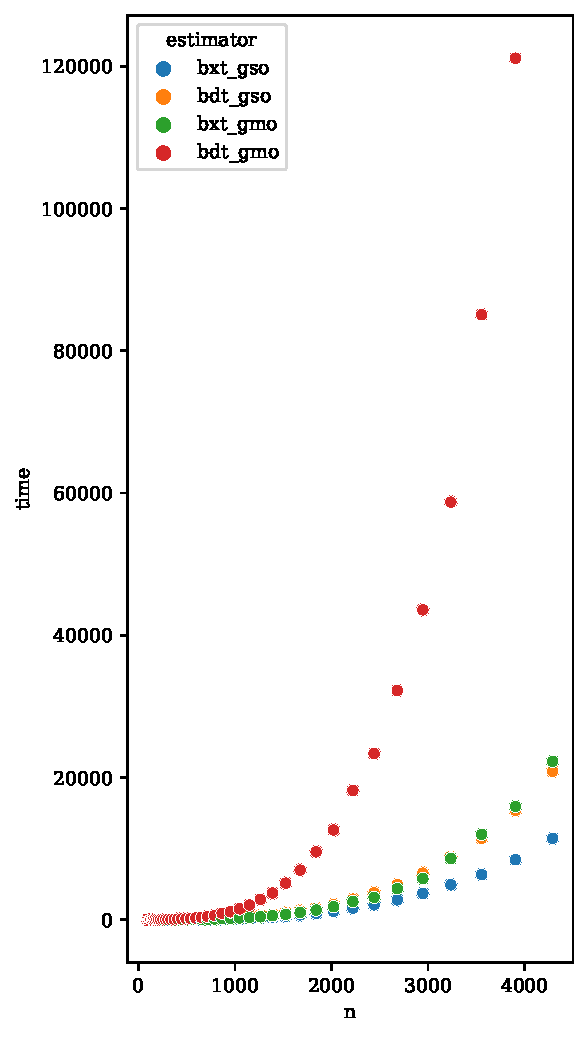
\includegraphics[width=\textwidth]{
            experiments/empirical_complexity/time_vs_n_artificial_data.pdf
        }
        \caption{Training durations in seconds versus the the number of samples and features.}
    \end{subfigure}
    \begin{subfigure}{0.49\textwidth}
        \includegraphics[width=\textwidth]{
            experiments/empirical_complexity/%
            time_vs_n_artificial_data_loglog.pdf
        }
        \caption{Logarithm of the training durations in seconds versus the logarithm of the number of samples and features.}
    \end{subfigure}
    \caption{
        Empirical time complexity estimation of the proposed bipartite global single-output (BGSO) and the global multi-output (GMO)~\cite{pliakos2018}
        algorithms. Bipartite versions of both extremely randomized trees~\cite{geurts2006extremely} (BXT) and greedy decision trees~\cite{breiman1984} (BDT) were built under the GSO and GMO scheme and trained over artificial datasets of varying numbers of samples (as described in section \ref{sec:complexity_analysis}). Applying least-squares linear regression to the logarithm of the values in (a), as shown in (b), the empirical slopes and respective standard deviations are obtained.
        Independent two-sample t-tests comparing the slope estimates reveal that the time complexity of \texttt{bdt\_gso} is highly significantly lower than \texttt{bdt\_gmo} (p-value $< 10^{-64}$) and even \texttt{bxt\_gmo} (p-value $< 10^{-20}$), and also that \texttt{bxt\_gso} significantly exhibits lower complexity than \texttt{bxt\_gmo} (p-value $< 10^{-22}$). Those values
        corroborate the theoretical estimates from section \ref{sec:complexity_analysis}.
    }
    \label{fig:empirical_complexity}
\end{figure}


\subsection{Comparison between GSO models}  % TODO

To assess the impact of global single-output optimizations in bipartite decision tree growing, we compare three slightly different training methods for BXT and BRF models.

\begin{itemize}
    \item \textbf{ngso}: Naive global single output implementation (Section \ref{});
    \item \textbf{ngsous}: Naive global single output implementation with undersampling of the non-interacting pairs to yield a balanced training set (Section \ref{});
    \item \textbf{gso}: Optimized implementation of global single output trees (Section \ref{}).
\end{itemize}

While no significant divergence was measured among the GSO models using the entirety of the training data, undersampling revealed to significantly degrade the predictive performance of both forests in terms of AUPR and MCC (Figure \ref{fig:cdd_gso_models}), eventhough it is arguably the most common procedure when dealing with this kind of data \cite{}.

On the other hand, AUROC is significantly improved by the undersampling procedure, which is most likely an artifact of the highly imbalanced nature of the present data, as explained as follows. The models grown on the undersampled datasets are naturally the most likely to assign positive labels to new interactions in general, improving TPR at the expense of also increasing FPR. However, since negative labels greatly outnumbers positive labels in the test sets of our current scenario, an increase in FPR impacts a much larger number of predictions than the same increase in TPR. In spite of that, AUROC equally treats TPR and FPR, so that the impact of a high FPR is underestimated. As such, AUROC results could be deemed as unrepresentative of model performance in this setup.

% \begin{figure*}
%     \centering
%     \begin{subfigure}{0.32\textwidth}
%         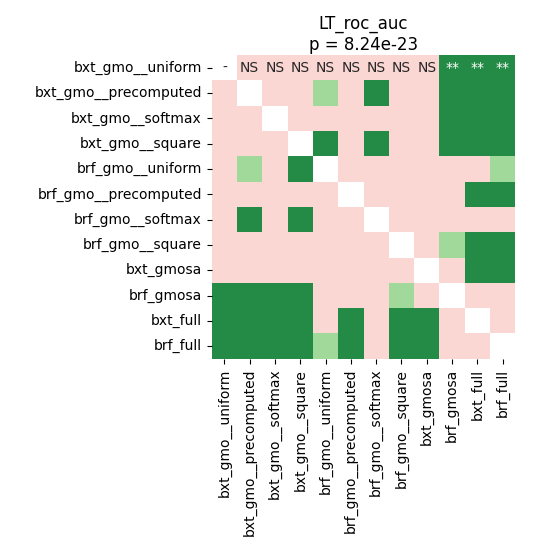
\includegraphics[width=\textwidth]{
%             experiments/gso_optimization/figures/%
%             estimator_name/enzymes__LT_roc_auc.pdf
%         }
%     \end{subfigure}
%     \begin{subfigure}{0.32\textwidth}
%         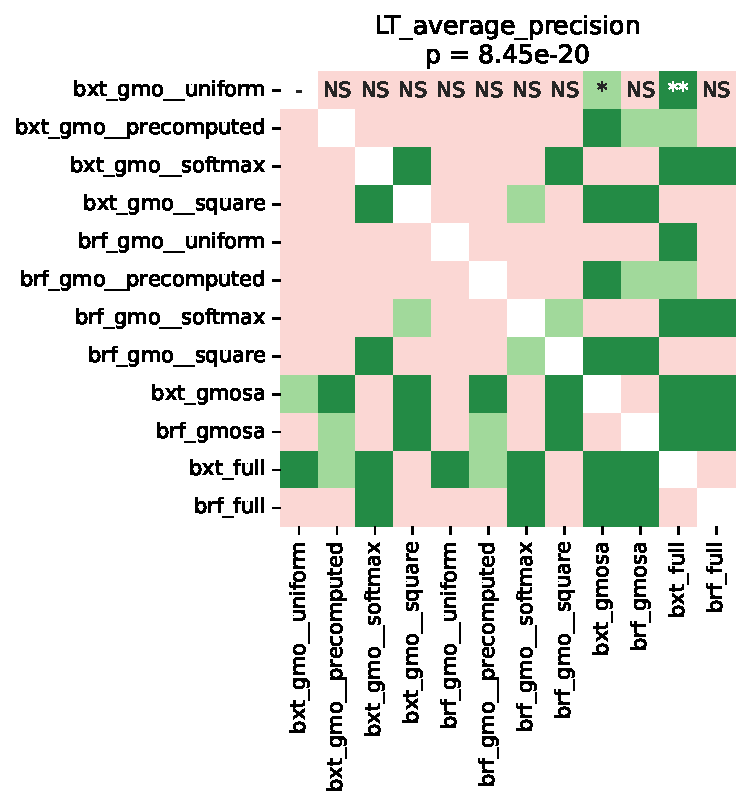
\includegraphics[width=\textwidth]{
%             experiments/gso_optimization/figures/%
%             estimator_name/enzymes__LT_average_precision.pdf
%         }
%     \end{subfigure}
%     \begin{subfigure}{0.32\textwidth}
%         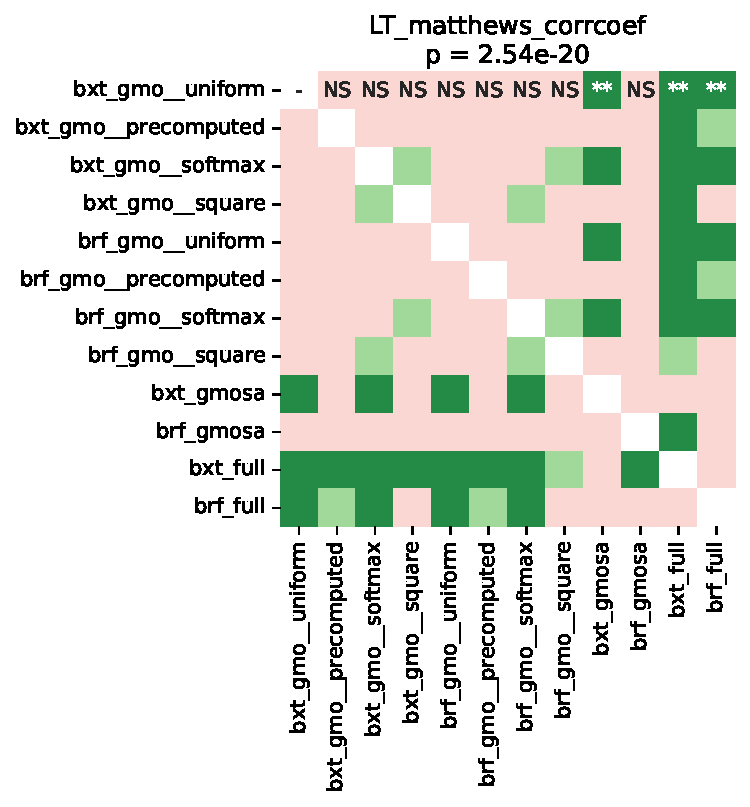
\includegraphics[width=\textwidth]{
%             experiments/gso_optimization/figures/%
%             estimator_name/enzymes__LT_matthews_corrcoef.pdf
%         }
%     \end{subfigure}
% 
%     \begin{subfigure}{0.32\textwidth}
%         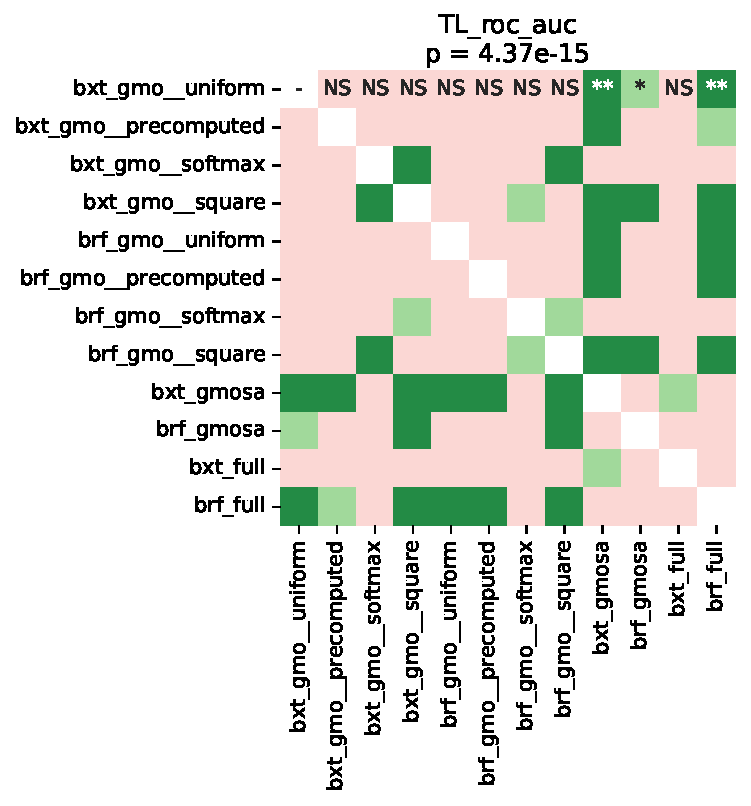
\includegraphics[width=\textwidth]{
%             experiments/gso_optimization/figures/%
%             estimator_name/enzymes__TL_roc_auc.pdf
%         }
%     \end{subfigure}
%     \begin{subfigure}{0.32\textwidth}
%         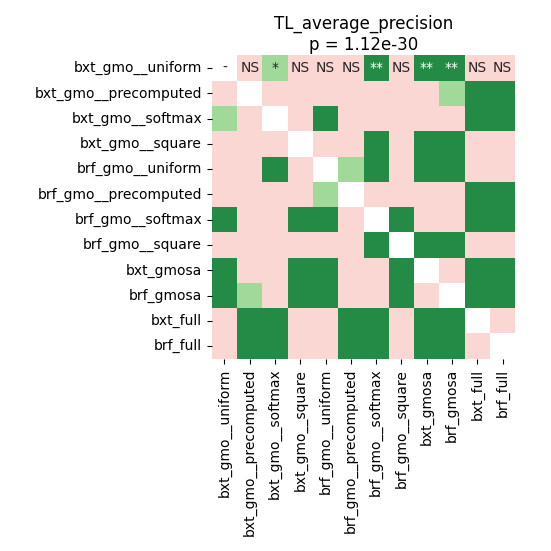
\includegraphics[width=\textwidth]{
%             experiments/gso_optimization/figures/%
%             estimator_name/enzymes__TL_average_precision.pdf
%         }
%     \end{subfigure}
%     \begin{subfigure}{0.32\textwidth}
%         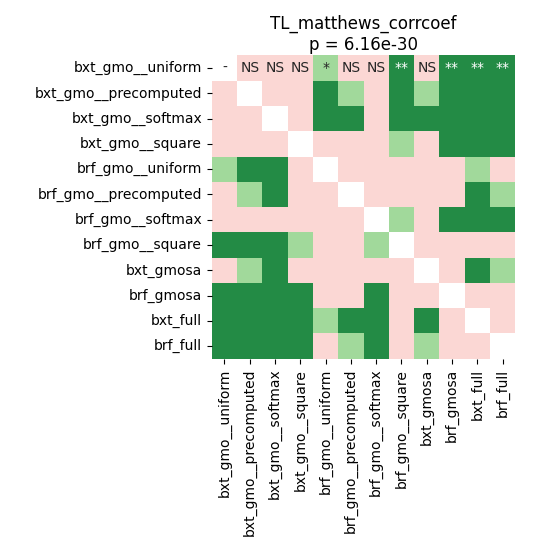
\includegraphics[width=\textwidth]{
%             experiments/gso_optimization/figures/%
%             estimator_name/enzymes__TL_matthews_corrcoef.pdf
%         }
%     \end{subfigure}
% 
%     \begin{subfigure}{0.32\textwidth}
%         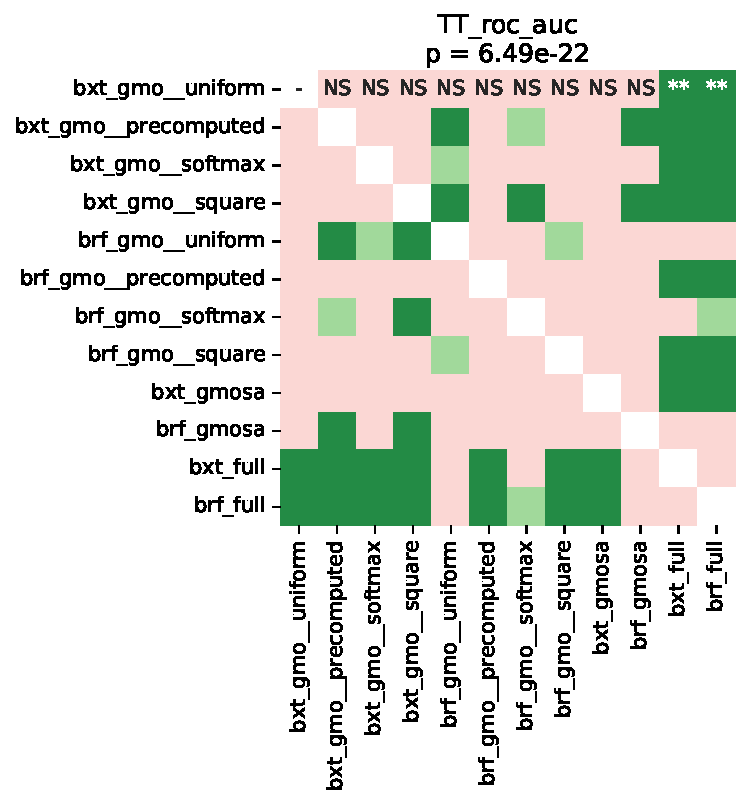
\includegraphics[width=\textwidth]{
%             experiments/gso_optimization/figures/%
%             estimator_name/enzymes__TT_roc_auc.pdf
%         }
%     \end{subfigure}
%     \begin{subfigure}{0.32\textwidth}
%         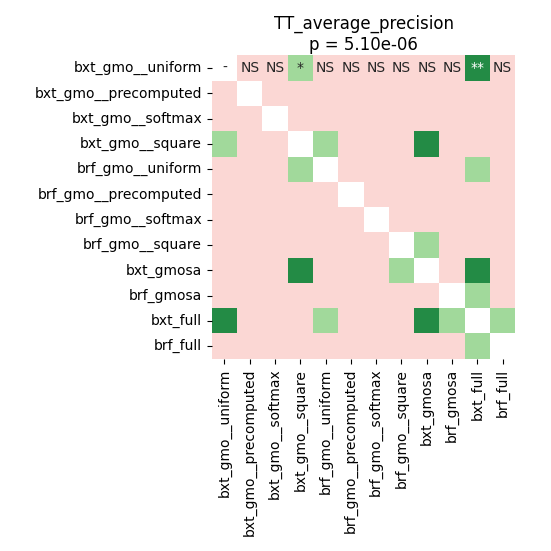
\includegraphics[width=\textwidth]{
%             experiments/gso_optimization/figures/%
%             estimator_name/enzymes__TT_average_precision.pdf
%         }
%     \end{subfigure}
%     \begin{subfigure}{0.32\textwidth}
%         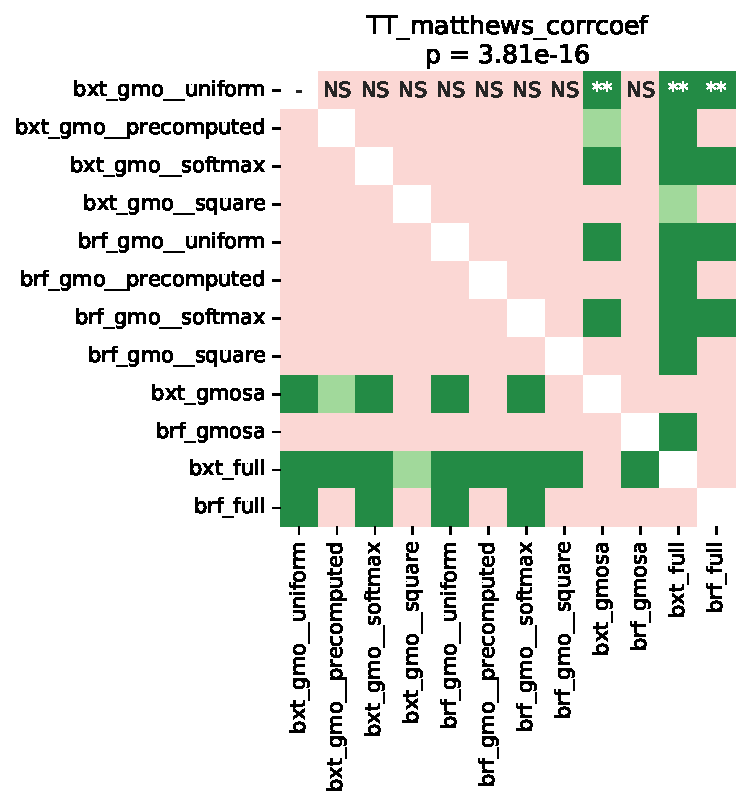
\includegraphics[width=\textwidth]{
%             experiments/gso_optimization/figures/%
%             estimator_name/enzymes__TT_matthews_corrcoef.pdf
%         }
%     \end{subfigure}
%     \caption{Comparison between GSO models on the Enzymes dataset.}
%     \label{fig:box_\text{SGSO}so_models_enzymes}
% \end{figure*}
% 
% 
% \begin{figure*}
%     \centering
%     \begin{subfigure}{0.32\textwidth}
%         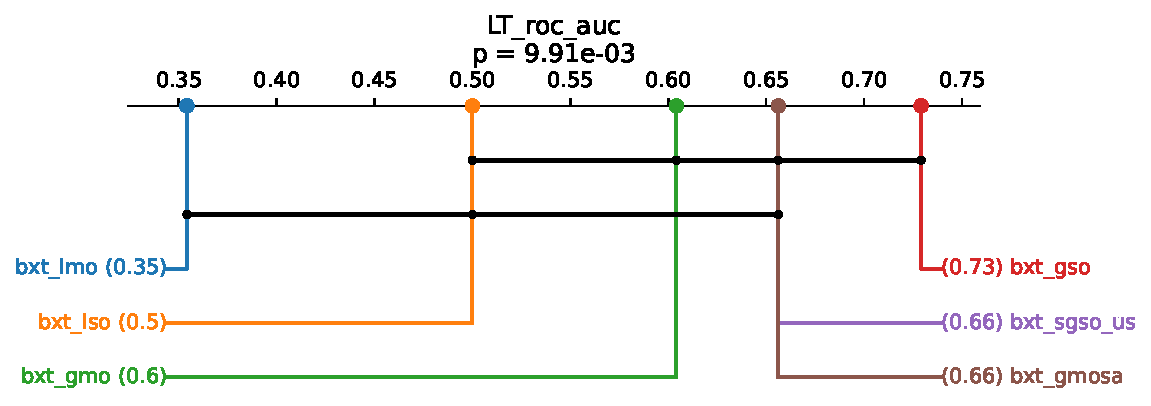
\includegraphics[width=\textwidth]{
%             experiments/gso_optimization/statistical_comparisons/%
%             all_datasets/critical_difference_diagrams/LT_roc_auc.pdf
%         }
%     \end{subfigure}
%     \begin{subfigure}{0.32\textwidth}
%         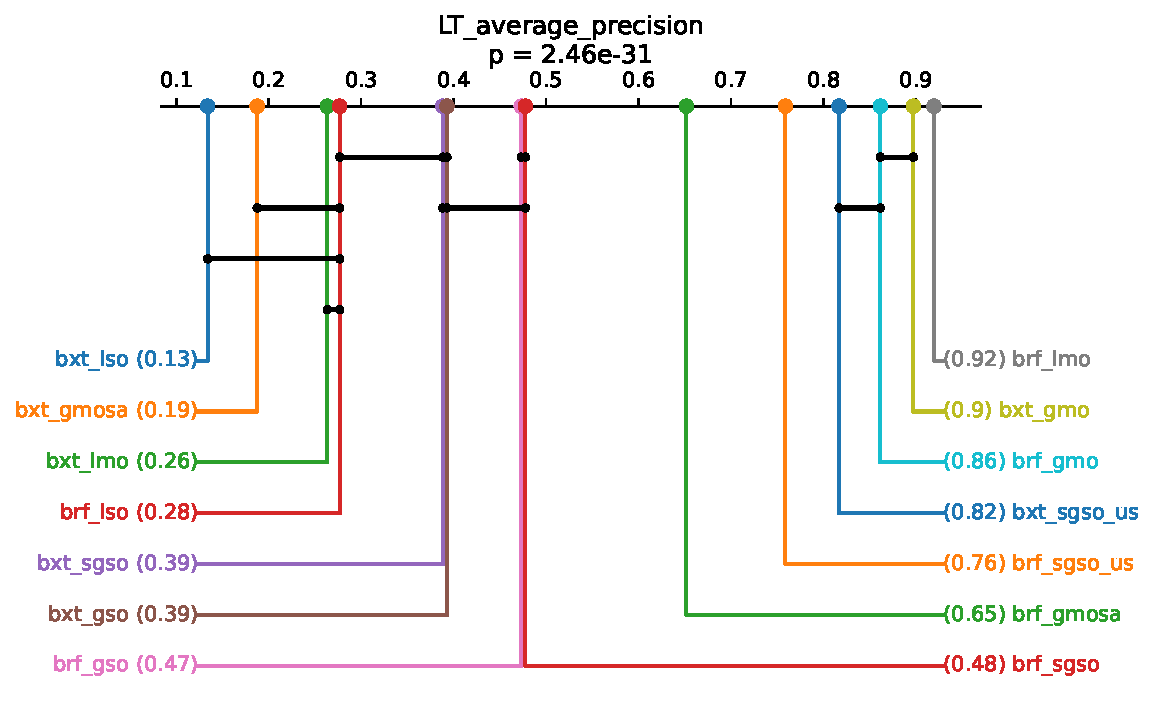
\includegraphics[width=\textwidth]{
%             experiments/gso_optimization/statistical_comparisons/%
%             all_datasets/critical_difference_diagrams/LT_average_precision.pdf
%         }
%     \end{subfigure}
%     \begin{subfigure}{0.32\textwidth}
%         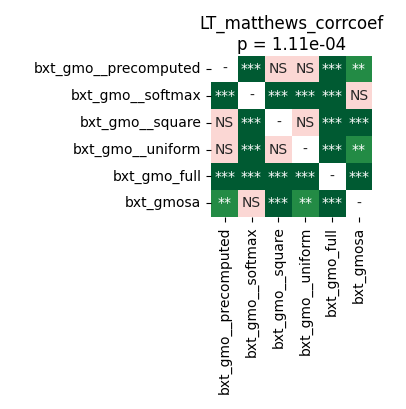
\includegraphics[width=\textwidth]{
%             experiments/gso_optimization/statistical_comparisons/%
%             all_datasets/critical_difference_diagrams/LT_matthews_corrcoef.pdf
%         }
%     \end{subfigure}
% 
%     \begin{subfigure}{0.32\textwidth}
%         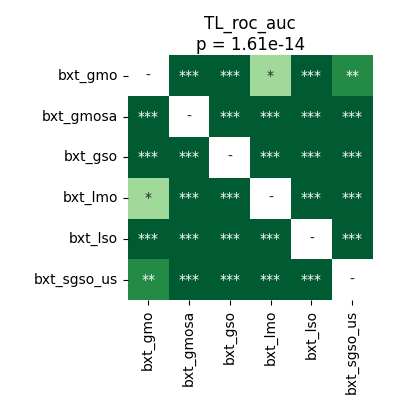
\includegraphics[width=\textwidth]{
%             experiments/gso_optimization/statistical_comparisons/%
%             all_datasets/critical_difference_diagrams/TL_roc_auc.pdf
%         }
%     \end{subfigure}
%     \begin{subfigure}{0.32\textwidth}
%         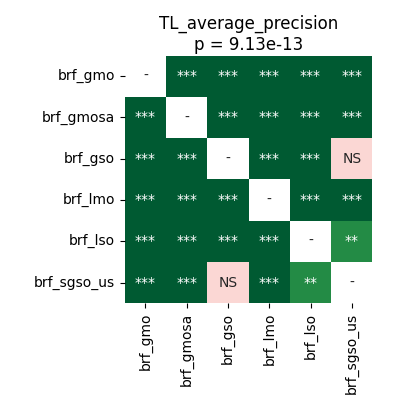
\includegraphics[width=\textwidth]{
%             experiments/gso_optimization/statistical_comparisons/%
%             all_datasets/critical_difference_diagrams/TL_average_precision.pdf
%         }
%     \end{subfigure}
%     \begin{subfigure}{0.32\textwidth}
%         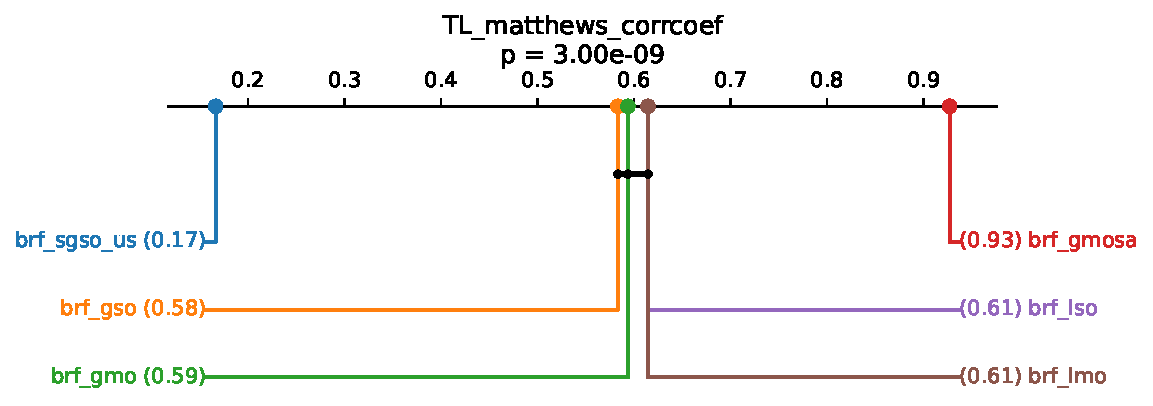
\includegraphics[width=\textwidth]{
%             experiments/gso_optimization/statistical_comparisons/%
%             all_datasets/critical_difference_diagrams/TL_matthews_corrcoef.pdf
%         }
%     \end{subfigure}
% 
%     \begin{subfigure}{0.32\textwidth}
%         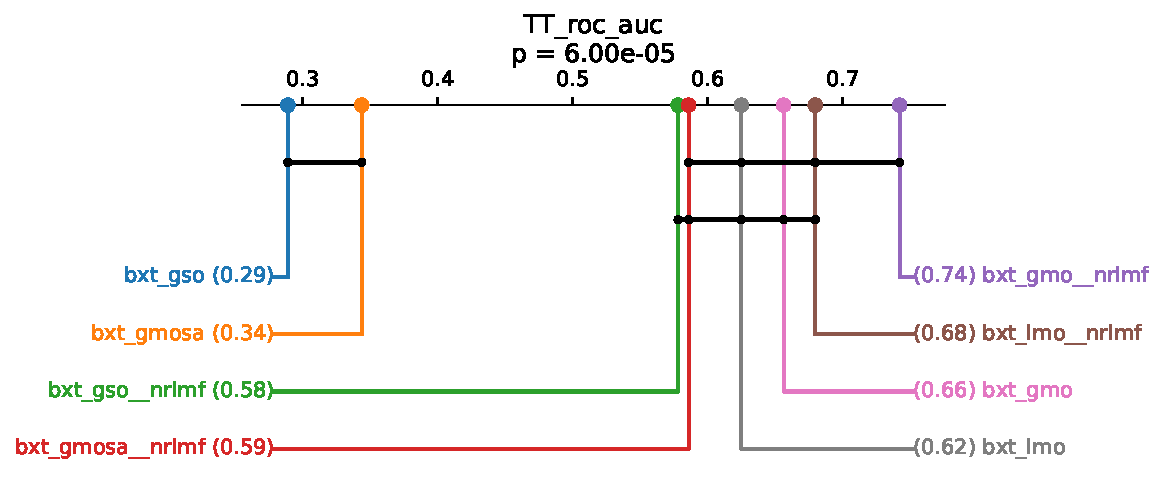
\includegraphics[width=\textwidth]{
%             experiments/gso_optimization/statistical_comparisons/%
%             all_datasets/critical_difference_diagrams/TT_roc_auc.pdf
%         }
%     \end{subfigure}
%     \begin{subfigure}{0.32\textwidth}
%         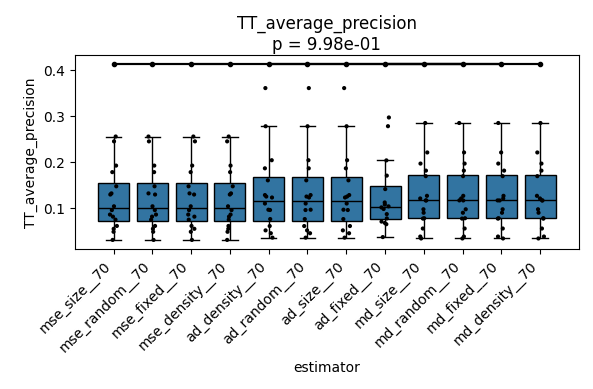
\includegraphics[width=\textwidth]{
%             experiments/gso_optimization/statistical_comparisons/%
%             all_datasets/critical_difference_diagrams/TT_average_precision.pdf
%         }
%     \end{subfigure}
%     \begin{subfigure}{0.32\textwidth}
%         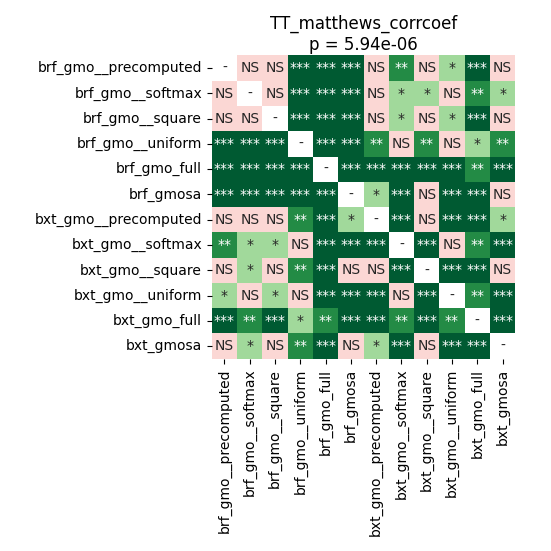
\includegraphics[width=\textwidth]{
%             experiments/gso_optimization/statistical_comparisons/%
%             all_datasets/critical_difference_diagrams/TT_matthews_corrcoef.pdf
%         }
%     \end{subfigure}
%     \caption{Percentile rankings of prediction scores for each global single output strategy.}
%     \label{fig:cdd_gso_models}
% \end{figure*}

% TODO: talk about pairwise CV

When comparing training times, the common choice for undersampling in previous works is justified, as an expressive reduction of training time is observed for both forests (Table \ref{}) relative to naive GSO training. Nevertheless, it is remarkable that the optimized implementation of GSO forests achieves similar training times in comparison to undersampled GSO without the AUPR and MCC burden of undersampling, keeping the higher scores resulting from employing the entirety of the dataset. For larger and less imbalanced datasets, the optimized implementation of GSO forests is expected to be even more advantageous, in agreement with the theoretical time complexity analysis (Section \ref{}).

%\begin{table}[h]
%    \input{
%        figures/experiments/gso_optimization/%
%        latex_tables/fit.tex
%    }
%\end{table}

In conclusion, the proposed approach confidently enables the use of the entire training data in a much shorter time frame than naive implementations without the need for data undersampling, which is statistically expected to yield better prediction scores for forest predictors.


\subsection{Comparison between GMO prediction weights}
\label{sec:prototype_comparison}
%TODO: why we did not use BGSO here?

In this work we propose a different prototyping strategy to determine the output value of each leaf in a GMO decision tree, taking the similarity matrices of our use cases into consideration (\autoref{sec:prototype}).

We here compare such strategies, building BXT and BRF models for every option. The minimum rows per leaf and minimum columns per leaf were both set to 5, ensuring a minimum number of co-leaf samples of each domain to be considered in a weighted-neighbors fashion during evaluation (Section \ref{}).

To take the effect of the early-stopping criterion into account (minimum number of samples in each leaf), we also include forests of fully-grown trees in the comparison. The compared models are described below.

\begin{itemize}
    \item \textbf{\texttt{gmosa}:} proposed by \textcite{pliakos2018global}, the output of each leaf is the average of the labels of the learned samples that reach that leaf (\autoref{eq:prototype1}).
    \item \textbf{\texttt{uniform}:} also proposed by \textcite{pliakos2018global}, the only difference from the \texttt{gmosa} strategy occurs in TL or LT test settings, when the average is taken only among the labels of the known sample of the pair being predicted (\autoref{eq:prototype2}).
    \item \textbf{\texttt{precomputed}:} introduced by us (as also \texttt{square} and \texttt{softmax}), the labels in each leaf are weighted by the similarities between the learned samples and the pair being predicted (\autoref{eq:prototype3}).
    \item \textbf{\texttt{square}:} the labels in each leaf are weighted by the squared similarities between the learned samples and the pair being predicted (\autoref{eq:prototype3}).
    \item \textbf{\texttt{softmax}:} the labels in each leaf are weighted by the exponential of the similarities between the learned samples and the pair being predicted (\autoref{eq:prototype3}).
    \item \textbf{\texttt{full}:} the trees are grown until a single interaction remains in each leaf. %, so that the prediction for each pair is the label of the single learned sample in the leaf.
\end{itemize}

%As shown by \autoref{fig:pred_weights_brf} and Table \ref{}, BXT models show an overall superior performance in comparison to BRF models, with each BXT model scoring significantly higher than its BRF counterpart with the same prediction weights. Furthermore, the weighted GMO predictions seem to prevail relative to the leaf-wise prototype GMOSA (Section \ref{}). Specifically, bxt\_square significantly outperforms all other bipartite forests except for bxt\_precomputed, both in terms of AUROC and average precision (AUPR) in the TT sets (Figure \ref{}).

The results for BRF (\autoref{fig:pred_weights_brf}) and BXT (\autoref{fig:pred_weights_bxt}) were similar. In all cases except LT+TL average precision, using the square of the similarities to weight the labels in each leaf resulted in significantly better scores than all other options. For the LT+TL average precision score, growing the decision tree to its maximal size emerged as the best strategy, followed by \texttt{uniform}, the original proposal by \textcite{pliakos2018global} of averaging only the 
outputs of the learned samples (known from the training set) in each leaf. Another exception occurs for the LT+TL AUROC score of BRF, in which case the \texttt{uniform} strategy could not be statistically distinguished from the squared-similarities weighting approach, with both still displaying the best performances against the remaining models.

The fully-grown versions of both forest algorithms are shown to be especially advantageous when considering the LT+TL average precision, even more so regarding BXT, where their superiority is remarkably clear (\autoref{fig:pred_weights_bxt}). This suggests that building trees to their maximum depth is the best strategy for tackling mixed train-test tasks such as drug repositioning~\cite{}, even in comparison to the weighted GMO predictions proposed by \textcite{pliakos2018global} and by the present work to approach these scenarios. 

The maximum depth, however, may impact the model's generalization ability, since the same superiority is not shown for the TT average precision score, where both entities of the pair being predicted are unknown to the model. Our squared-similarity weights seemingly display the best generalization in this regard.

% TODO: why fully grown is not that good for AUROC
%The full models are also seemingly affected

% FIXME: gmosa vs gmo uniform on TT: indicates there are duplicated samples in the dataset, so training samples are leaking to test set.
We then select the squared-similarities model for the downstream analyses, keeping 5 by 5 as the minimum leaf partition size. While GMOSA will also be further investigated, the leaf size constraint will be dropped, generating fully-grown trees for this strategy hereafter.

\begin{figure*}[tbh]
    \centering
    \begin{subfigure}{0.49\textwidth}
        \includegraphics[width=\textwidth]{
            experiments/prediction_weights/statistical_comparisons/%
            brf/all_datasets/boxplots/LT+TL_roc_auc.pdf
        }
    \end{subfigure}
    \begin{subfigure}{0.49\textwidth}
        \includegraphics[width=\textwidth]{
            experiments/prediction_weights/statistical_comparisons/%
            brf/all_datasets/boxplots/LT+TL_average_precision.pdf
        }
    \end{subfigure}

    \begin{subfigure}{0.49\textwidth}
        \includegraphics[width=\textwidth]{
            experiments/prediction_weights/statistical_comparisons/%
            brf/all_datasets/boxplots/TT_roc_auc.pdf
        }
    \end{subfigure}
    \begin{subfigure}{0.49\textwidth}
        \includegraphics[width=\textwidth]{
            experiments/prediction_weights/statistical_comparisons/%
            brf/all_datasets/boxplots/TT_average_precision.pdf
        }
    \end{subfigure}
    \caption{
        Percentile rankings of prediction scores of bipartite random forests for different prediction weighting strategies, across all 10 datasets.
        The omnibus p-value obtained through a Friedman test is indicated below each plot's title. Significant results in each case lead us to perform pairwise Wilcoxon rank-sum tests, whose non-significant results are indicated by crossbars above each plot, that is, statistically undistinguished boxes are connected by the crossbars. The pairwise test results were corrected by the Benjamini-Hochberg procedure among each subfigure, considering that all possible estimator pairs were evaluated even if their comparison is not indicated in the plot. See \autoref{sec:empirical_complexity} for further descriptions of each estimator.
    }
    \label{fig:pred_weights_brf}
\end{figure*}


\begin{figure*}[tbh]
    \centering
    \begin{subfigure}{0.49\textwidth}
        \includegraphics[width=\textwidth]{
            experiments/prediction_weights/statistical_comparisons/%
            bxt/all_datasets/boxplots/LT+TL_roc_auc.pdf
        }
    \end{subfigure}
    \begin{subfigure}{0.49\textwidth}
        \includegraphics[width=\textwidth]{
            experiments/prediction_weights/statistical_comparisons/%
            bxt/all_datasets/boxplots/LT+TL_average_precision.pdf
        }
    \end{subfigure}

    \begin{subfigure}{0.49\textwidth}
        \includegraphics[width=\textwidth]{
            experiments/prediction_weights/statistical_comparisons/%
            bxt/all_datasets/boxplots/TT_roc_auc.pdf
        }
    \end{subfigure}
    \begin{subfigure}{0.49\textwidth}
        \includegraphics[width=\textwidth]{
            experiments/prediction_weights/statistical_comparisons/%
            bxt/all_datasets/boxplots/TT_average_precision.pdf
        }
    \end{subfigure}
    \caption{
        Percentile rankings of prediction scores of bipartite extremely randomized trees for different prediction weighting strategies, across all 10 datasets.
        The omnibus p-value obtained through a Friedman test is indicated below each plot's title. Significant results in each case lead us to perform pairwise Wilcoxon rank-sum tests, whose non-significant results are indicated by crossbars above each plot, that is, statistically undistinguished boxes are connected by the crossbars. The pairwise test results were corrected by the Benjamini-Hochberg procedure among each subfigure, considering that all possible estimator pairs were evaluated even if their comparison is not indicated in the plot. See \autoref{sec:empirical_complexity} for further descriptions of each estimator.
    }
    \label{fig:pred_weights_bxt}
\end{figure*}


\subsection{Comparison between adaptation strategies}
\label{sec:adaptation_comparison}

Still restricted to forest estimators, we compare each of the described approaches for adapting models to bipartite data (\autoref{sec:common_approaches}, \autoref{sec:bipartite_trees} and \autoref{sec:bgso_trees}). The suffixes in the model names of this section indicating the employed bipartite adaptations are briefly described below.

% TODO: contribution: ensembles of gmo (not gmosa) were nevel built!

\begin{itemize}
    \item \textbf{\texttt{lmo}:} implements the standard local multi-output approach (SLMO; \autoref{sec:slmo}) by training four separate multioutput models, two for each domain. First explored by \textcite{schrynemackers2015classifying}.
    \item \textbf{\texttt{lso}:} also implements the SLMO approach (\autoref{sec:slmo}), but each multioutput model is instead a composition of several local single-output (LSO) models, i.e. one model is trained for each row or column of the interaction matrix. This setting is similar to the early proposal by \textcite{bleakley2009supervised}, but employing decision forests as the base algorithm.
    \item \textbf{\texttt{gmosa}:} a global multi-output forest with single-label averaging (GMOSA; \autoref{sec:gmo}), as explored by \textcite{pliakos2019network} under the name eBICT.
    \item \textbf{\texttt{gmo}:} a global multi-output (GMO; \autoref{sec:gmo}) forest with minimum leaf dimensions of 5 by 5, implementing our proposed squared-similarities weighting for the prototype function (\autoref{sec:prototype}). Apart from the new prototype, this model is based on the original GMO trees proposed by \textcite{pliakos2018global}. Despite their original results suggesting advantage over GMOSA, to the best of our knowledge, this is the first time the GMO trees are employed in building decision forests.  % TODO explain GMOSA
    \item \textbf{\texttt{gso}:} a bipartite global single-output (BGSO; \autoref{sec:bgso}) forest, as initially explored by \textcite{schrynemackers2015classifying} but now implementing our proposed algorithm with improved computational complexity.
    \item \textbf{\texttt{sgso\_us}:} implements the standard global single-output (SGSO; \autoref{sec:sgso}) adaptation, additionally employing undersampling of the non-interacting pairs to yield a balanced training set (\autoref{sec:sgso}).  % TODO explain that is frequently used
\end{itemize}

All the global models were built with 100 trees. For SLMO, each of the four forests used 50 trees, while for LSO 50 trees were used for each row or column of the interaction matrix.

Regarding BRF models, SLMO and GMO reveal themselves as the top-scoring adaptations. In the LT+TL setting, SLMO significantly outperforms all other models. In the TT test sets, SLMO was the second best-ranked model, significantly surpassing all models except LSO, SGSOUS and GMO. GMO, in turn, outshines all the remaining models in the TT setting.

The GMO approach is also highlighted by the results of BXT ensembles, being undisputed for the LT+TL AUROC and TT scores. Interestingly, for the LT+TL average precision score, its mean percentile ranking was the second to last, being only better than SGSOUS. These results corroborate the idea discussed in \autoref{sec:prototype_comparison} that reaching the maximum tree depth is the best strategy for LT+TL, while enforcing larger leaves and label weighting seems to improve generalization to unseen instances.

% TODO advantage of BGSOUS in AUROC
% TODO training times

% To avoid differences in random sampling when using the naive GSO adapter versus the natively bipartite GSO tree, no bootstraping was applied to any forest, providing all trees with the whole training samples space. To still ensure randomization in random forest estimators, the maximum features parameter was set to $0.5$, meaning that each tree in a random forest was trained on a random subset of half the features from each sample domain. Due to implementation details, this means the naive GSO forests will sample features slightly differently: they will pick half the features from the whole feature space combined, while the natively bipartite GSO forests will ensure half the features from each sample domain is selected. This is not expected to have a significant impact on the results, given that the total number of features is especially high in the present scenario, where similarity matrices are being employed. 

%All forests were composed of 100 tree estimators and were fully grown, with the exception of the GMO models, whose leaf sizes were limited to a minimum of 5 by 5 samples (at least 5 samples from each domain) in order to take advantage of neighborhood weighting (which was set to the squared similarities, see Section \ref{}).

%In all of the evaluated scenarios, a BXT model was ranked the best. In both TT-MCC and TL-AP, the BRF models and bxt\_gmo were significantly surpassed by the remaining BXT forests. In TL-MCC, bxt\_lso significantly outperformed all the other models. Given that this test-set provides the greatest intersection with the training set, due to the overall higher number of column samples in the datasets we used, we suggest that the LSO model could be better at taking advantage of already seen information from a sample domain, since a forest is grown separately for each row and column. From another perspective, this effect could be regarded as a form of overfitting. This hypothesis is further supported by the fact that both GMO models, which were the only forests subject to a minimum leaf size constraint and thus less prone, in theory, to overfitting, were the most frequently outperformed models in the TL-MCC and TL-AP.

%Contrastingly, both GMO models were consistently the best performing models in all AUROC settings, which is commonly assumed to be a less indicative metric in highly imbalanced classification contexts such as the present one \cite{}. This could be explained by a bias towards the majority class, possibly caused by the averaging of the larger leaves employed in this methods. %FIXME: actually, a bias towards minority class

\begin{figure*}[tbh]
    \centering
    \begin{subfigure}{0.49\textwidth}
        \includegraphics[width=\textwidth]{
            experiments/bipartite_adaptations/statistical_comparisons/%
            brf/all_datasets/boxplots/LT+TL_roc_auc.pdf
        }
    \end{subfigure}
    \begin{subfigure}{0.49\textwidth}
        \includegraphics[width=\textwidth]{
            experiments/bipartite_adaptations/statistical_comparisons/%
            brf/all_datasets/boxplots/LT+TL_average_precision.pdf
        }
    \end{subfigure}

    \begin{subfigure}{0.49\textwidth}
        \includegraphics[width=\textwidth]{
            experiments/bipartite_adaptations/statistical_comparisons/%
            brf/all_datasets/boxplots/TT_roc_auc.pdf
        }
    \end{subfigure}
    \begin{subfigure}{0.49\textwidth}
        \includegraphics[width=\textwidth]{
            experiments/bipartite_adaptations/statistical_comparisons/%
            brf/all_datasets/boxplots/TT_average_precision.pdf
        }
    \end{subfigure}
    \caption{
        Percentile rankings of prediction scores of random forest models under different adaptation strategies to bipartite interaction data, across all 10 datasets.
        The omnibus p-value obtained through a Friedman test is indicated below each plot's title. Significant results in each case lead us to perform pairwise Wilcoxon rank-sum tests, whose non-significant results are indicated by crossbars above each plot, that is, statistically undistinguished boxes are connected by the crossbars. The pairwise test results were corrected by the Benjamini-Hochberg procedure among each subfigure, considering that all possible estimator pairs were evaluated even if their comparison is not indicated in the plot. See \autoref{sec:adaptation_comparison} for further descriptions of each estimator.
    }
    \label{fig:adaptations_brf}
\end{figure*}


\begin{figure*}[tbh]
    \centering
    \begin{subfigure}{0.49\textwidth}
        \includegraphics[width=\textwidth]{
            experiments/bipartite_adaptations/statistical_comparisons/%
            bxt/all_datasets/boxplots/LT+TL_roc_auc.pdf
        }
    \end{subfigure}
    \begin{subfigure}{0.49\textwidth}
        \includegraphics[width=\textwidth]{
            experiments/bipartite_adaptations/statistical_comparisons/%
            bxt/all_datasets/boxplots/LT+TL_average_precision.pdf
        }
    \end{subfigure}

    \begin{subfigure}{0.49\textwidth}
        \includegraphics[width=\textwidth]{
            experiments/bipartite_adaptations/statistical_comparisons/%
            bxt/all_datasets/boxplots/TT_roc_auc.pdf
        }
    \end{subfigure}
    \begin{subfigure}{0.49\textwidth}
        \includegraphics[width=\textwidth]{
            experiments/bipartite_adaptations/statistical_comparisons/%
            bxt/all_datasets/boxplots/TT_average_precision.pdf
        }
    \end{subfigure}
    \caption{
        Percentile rankings of prediction scores of extremely randomized tree ensembles under different adaptation strategies to bipartite interaction data, across all 10 datasets.
        The omnibus p-value obtained through a Friedman test is indicated below each plot's title. Significant results in each case lead us to perform pairwise Wilcoxon rank-sum tests, whose non-significant results are indicated by crossbars above each plot, that is, statistically undistinguished boxes are connected by the crossbars. The pairwise test results were corrected by the Benjamini-Hochberg procedure among each subfigure, considering that all possible estimator pairs were evaluated even if their comparison is not indicated in the plot. See \autoref{sec:adaptation_comparison} for further descriptions of each estimator.
    }
    \label{fig:adaptations_bxt}
\end{figure*}


\subsection{Effect of interaction matrix reconstruction}

It was previously suggested that employing logistic matrix factorization to create a denser representation of the interaction matrix and using this representation as the training data for a BXT forest could improve their performance on DTI datasets \cite{Pliakos_2020}. To test this hypothesis, we compare the bipartite forests cross-validation scores with and without the interaction matrix reconstruction step. As done by \cite{Pliakos_2020}, the reconstruction step was performed using neighborhood-regularized logistic matrix factorization (NRLMF)\cite{}. The results are shown in Figure \ref{fig:cdd_reconstruction}.

To select hyperparameters for the NRLMF algorithm, we performed a randomized search in which 100 different combinations of hyperparameters were evaluated in terms of their resulting mean squared error over a (nested) bipartite 5-fold diagnonal cross-validation. The best combination found in the inner CV loop was then used to reconstruct the interaction matrix of each outer CV fold, and the resulting matrices were used as the training data for the bipartite forests. Note that a single forest was built by outer CV fold, so that the NRLMF hyperparameter seach was performed independently to the downstream forest performance. The hyperparameters \texttt{lambda\_rows}, \texttt{lambda\_cols}, \texttt{alpha\_cols}, \texttt{alpha\_cols}, and \texttt{learning\_rate} were all independently sampled from a log-uniform distribution bounded by $\frac{1}{4}$ and $2$. the number of latent vector components were set to be equal among noth axes, and chosen between 50 and 100. The number of neighbors was randomly selected as 3, 5 or 10 in each iteration, and the maximum number of optimization steps was always set to 100.

The results are shown in Figure \ref{fig:cdd_reconstruction}.

In accordance to the previous findings of \cite{Pliakos_2020}, the models with output space reconstruction either show significantly higher AUROC and AUPR or generated inconclusive results regarding those metrics when compared to the models without the reconstruction by NRLMF.

Surprisingly, however, the MCC results tend to favor the opposite conclusion, with the models without reconstruction showing higher MCC scores in most cases.

% TODO: remake the following explanation after displaying the rank boxplots

A first explanation could be that the NRLMF hyperparameter search was not exhaustive enough, and that a better combination of hyperparameters could have been found. However, we later show in section \ref{} that the NRLMF model alone displays competitive performance, disfavoring such hypothesis of underfitting.

We also notice that \cite{Liu_2017} performs bipartite cross-validation in unusual fashion, by replacing with zeros the positive labels of pairs assigned to the test set but still using them to train the model. Albeit test labels are masked, each model thus still receives all available samples during training, and we hypothesize that unsupervised information from the test set could possibly still be exploited during training. For instance, estimating the sample density of the feature space could provide an importance score, a weight factor, for each sample, in order to favor correct predictions of denser clusters and undermine outliers. Wether and how this or similar mechanisms are explored by the NRLMF algorithm is out of the scope of this work, but we discourage the use of such CV strategy and point it as a possible reason for the higher NRLMF scores observed by previous authors \cite{Pliakos_2020;Liu_2017}.

% (False, they also used nested CV) The authors of \cite{Pliakos_2020} also do not clearly specify the could have employed the reconstruction step before splitting the data into the cross-validation folds, in which case the observed performance improvement could be attributed to indirect data leakage, where the labels used to train the downstream forest estimator were generated from neighbor samples that are possibly in the test sets.

\begin{figure*}
    \centering
    \begin{subfigure}{0.32\textwidth}
        \includegraphics[width=\textwidth]{
            experiments/y_reconstruction/figures/%
            estimator_name/all_datasets/boxplots/LT_roc_auc.pdf
        }
    \end{subfigure}
    \begin{subfigure}{0.32\textwidth}
        \includegraphics[width=\textwidth]{
            experiments/y_reconstruction/figures/%
            estimator_name/all_datasets/boxplots/LT_average_precision.pdf
        }
    \end{subfigure}
    \begin{subfigure}{0.32\textwidth}
        \includegraphics[width=\textwidth]{
            experiments/y_reconstruction/figures/%
            estimator_name/all_datasets/boxplots/LT_matthews_corrcoef.pdf
        }
    \end{subfigure}

    \begin{subfigure}{0.32\textwidth}
        \includegraphics[width=\textwidth]{
            experiments/y_reconstruction/figures/%
            estimator_name/all_datasets/boxplots/TL_roc_auc.pdf
        }
    \end{subfigure}
    \begin{subfigure}{0.32\textwidth}
        \includegraphics[width=\textwidth]{
            experiments/y_reconstruction/figures/%
            estimator_name/all_datasets/boxplots/TL_average_precision.pdf
        }
    \end{subfigure}
    \begin{subfigure}{0.32\textwidth}
        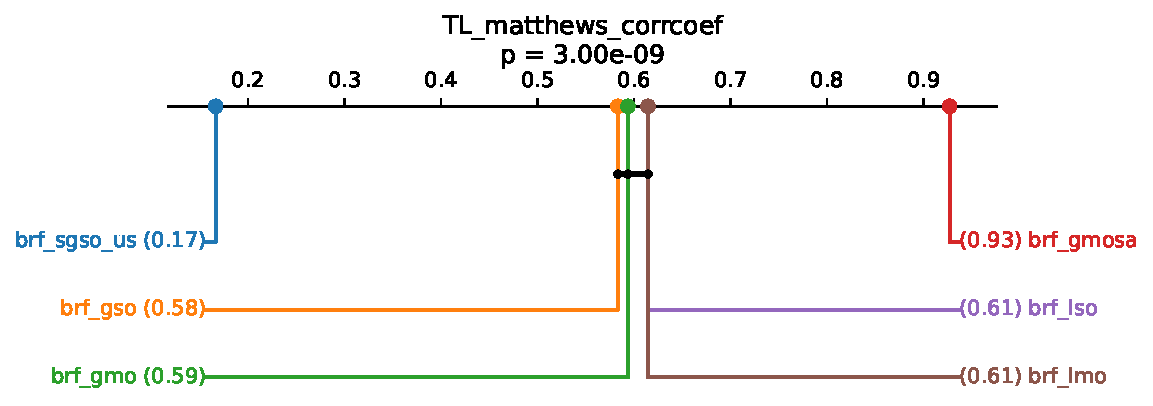
\includegraphics[width=\textwidth]{
            experiments/y_reconstruction/figures/%
            estimator_name/all_datasets/boxplots/TL_matthews_corrcoef.pdf
        }
    \end{subfigure}

    \begin{subfigure}{0.32\textwidth}
        \includegraphics[width=\textwidth]{
            experiments/y_reconstruction/figures/%
            estimator_name/all_datasets/boxplots/TT_roc_auc.pdf
        }
    \end{subfigure}
    \begin{subfigure}{0.32\textwidth}
        \includegraphics[width=\textwidth]{
            experiments/y_reconstruction/figures/%
            estimator_name/all_datasets/boxplots/TT_average_precision.pdf
        }
    \end{subfigure}
    \begin{subfigure}{0.32\textwidth}
        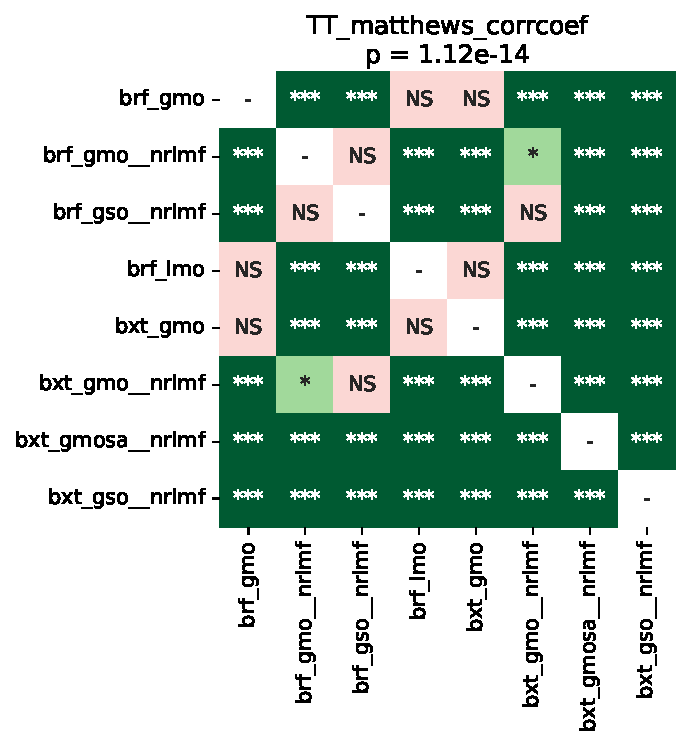
\includegraphics[width=\textwidth]{
            experiments/y_reconstruction/figures/%
            estimator_name/all_datasets/boxplots/TT_matthews_corrcoef.pdf
        }
    \end{subfigure}
    \caption{Comparison of scores for the bipartite forests with and without output space reconstruction on the enzymes dataset.}
    \label{fig:box_y_reconstruction}
\end{figure*}

% \begin{table}[h]
%     \input{figures/experiments/y_reconstruction/latex_tables/TT.tex}
% \end{table}


\subsection{Comparison with previous works}

In this section we employ several algorithms previously described in the literature, all of which were reimplemented and had their performance measured on the four DTI prediction datasets according to this study's evaluation framework (Section \ref{}).

The algorithms being considered in this section are listed below, and their scoring results are shown in Figure \ref{fig:cdd_literature} and Table \ref{}. To further explore the potential of bipartite forests, all forests evaluated in this section were composed of 1000 trees, as opposed to the 100 trees used in the previous experiments.

\begin{itemize}
    \item NRLMF \cite{Liu_2017}
    \item BLM-NII 
    % TODO
\end{itemize}

Regarding the AUROC metric, bxt\_gmosa\_nrlmf, bxt\_gso\_nrlmf and nrlmf are consistently the three highest ranked models in all three testing settings, with both bxt\_gmosa\_nrlmf and bxt\_gso\_nrlmf significantly outperforming BLM-NII-SVM, BLM-NII-RLS, and DTHybrid.
Additionally, DNILMF was outperformed by bxt\_gmosa\_nrlmf and bxt\_gso\_nrlmf in the TL and LT settings, and by bxt\_gmosa\_nrlmf in the TT setting.

Both in the LT and TT settings, the bipartite forests without matrix reconstruction (bxt\_gmosa and bxt\_gso) showed no significant difference in performance when compared to their counterparts employing interaction matrix reconstruction by NRLMF (bxt\_gmosa\_nrlmf and bxt\_gso\_nrlmf, respectively), contrary to the results on the TL testing configuration, where matrix reconstruction was shown to be significantly beneficial.
A possible explanation relies on the fact that the TL test set has the higher intersection with the training data in our specific scenario, since in the four datasets considered the drug molecules outnumber the protein targets by considerable margins (see Table \ref{tab:datasets}).
That said, NRLMF fundamentally relies on the label information of a small neighborhood of each sample to infer interactions and, as such, this result may suggest that the benefit of the matrix factorization step is elevated in cases where the test set is similar to the training set, and could be specifically useful in drug repurposing scenarios rather than in drug discovery. On the other hand, overfitting may arise as a potential concern when new drugs and new targets are of the main interest.

Additionally, one must recall we are using larger forests in comparison to the previous section, which may render the matrix factorization step less relevant.
This is further supported by the fact that the NRLMF model itself could not significantly outperform bxt\_gso in the LT\_roc\_auc setting, bxt\_gmosa in the TL\_roc\_auc setting and also could not outperform either forest in the TT\_roc\_auc setting (Figure \ref{fig:cdd_literature}), not ruling out the explanation that the tree ensemble itself is sufficient to encompass neighborhood information.

When the average precision metric is considered, the reconstruction step is again regarded unbeneficial, with no significant difference in employing it versus using the bipartite forest alone. Interestingly, all BXT forests perform significantly better than all other methods in the TL\_average\_precision setting, even than the matrix factorization techniques NRLMF and DNILMF (Figure \ref{fig:cdd_literature}). NRLMF, DNILMF and lmorls were the only methods not proven significantly inferior to the BXT in the remaining average precision settings. 

The superiority of DNILMF with respect to NRLMF as claimed by its authors \cite{} was not observed in our experiments, with NRLMF even proven significantly superior to DNILMF in the TL\_roc\_auc and LT\_roc\_auc settings (Figure \ref{fig:cdd_literature}).

With respect to the MCC metric, the bxt\_gmosa and bxt\_gso stand out as the best performing models, significantly outperforming all the other models in TL\_mcc, all but bxt\_gmosa\_nrlmf in LT\_mcc, and all but bxt\_gmosa\_nrlmf and bxt\_gso\_nrlmf in the TT setting.

However, this result is likely affected by the classification threshold choice, since this is the only metric we used that is threshold-dependent. Since we chose this threshold as the probability of interaction in each training set (the average of all binary values of $y$), the MCC metric will favor well calibrated models, i.e. whose predicted probabilities are close to the measured propabilities.  % TODO: define better and cite
As such, this result mainly indicates better calibration of the BXT models out of the box. Conversely, the other models may benefit from calibration techniques such as Platt scaling \cite{} or isotonic regression \cite{}, with BLM models being especially underperformant regarding MCC.

Overall, bxt\_gso and bxt\_gmosa are the most consistently higher ranked models among the algorithms we tested. Remarkably, we demonstrate in sections \ref{sec:complexity_analysis} and \ref{sec:empirical_complexity} that our optimized GSO forests are considerably faster to train than the GMO forests proposed by \cite{Pliakos_2018}, even if no statistically significant decrease in performance is observed. This time complexity superiority enables forest estimators to tackle much larger bipartite datasets than was possible with the current bipartite trees, and points native GSO bipartite forests as a strong candidate to be further studied across similar learning scenarios in the future.

\begin{figure*}
    \centering
    \begin{subfigure}{0.32\textwidth}
        \includegraphics[width=\textwidth]{
            experiments/literature_models/statistical_comparisons/%
            all_datasets/critical_difference_diagrams/LT_roc_auc.pdf
        }
    \end{subfigure}
    \begin{subfigure}{0.32\textwidth}
        \includegraphics[width=\textwidth]{
            experiments/literature_models/statistical_comparisons/%
            all_datasets/critical_difference_diagrams/LT_average_precision.pdf
        }
    \end{subfigure}
    \begin{subfigure}{0.32\textwidth}
        \includegraphics[width=\textwidth]{
            experiments/literature_models/statistical_comparisons/%
            all_datasets/critical_difference_diagrams/LT_matthews_corrcoef.pdf
        }
    \end{subfigure}

    \begin{subfigure}{0.32\textwidth}
        \includegraphics[width=\textwidth]{
            experiments/literature_models/statistical_comparisons/%
            all_datasets/critical_difference_diagrams/TL_roc_auc.pdf
        }
    \end{subfigure}
    \begin{subfigure}{0.32\textwidth}
        \includegraphics[width=\textwidth]{
            experiments/literature_models/statistical_comparisons/%
            all_datasets/critical_difference_diagrams/TL_average_precision.pdf
        }
    \end{subfigure}
    \begin{subfigure}{0.32\textwidth}
        \includegraphics[width=\textwidth]{
            experiments/literature_models/statistical_comparisons/%
            all_datasets/critical_difference_diagrams/TL_matthews_corrcoef.pdf
        }
    \end{subfigure}

    \begin{subfigure}{0.32\textwidth}
        \includegraphics[width=\textwidth]{
            experiments/literature_models/statistical_comparisons/%
            all_datasets/critical_difference_diagrams/TT_roc_auc.pdf
        }
    \end{subfigure}
    \begin{subfigure}{0.32\textwidth}
        \includegraphics[width=\textwidth]{
            experiments/literature_models/statistical_comparisons/%
            all_datasets/critical_difference_diagrams/TT_average_precision.pdf
        }
    \end{subfigure}
    \begin{subfigure}{0.32\textwidth}
        \includegraphics[width=\textwidth]{
            experiments/literature_models/statistical_comparisons/%
            all_datasets/critical_difference_diagrams/TT_matthews_corrcoef.pdf
        }
    \end{subfigure}
    \caption{Percentile rankings of prediction scores for several literature models.}
    \label{fig:cdd_literature}
\end{figure*}


% linear models underfitted. previous good results in TL an LT are likely partial data leakage due to network feature extraction

% even in TT, data leakage could occur if cv is performed by masking positives

% partial conclusions:
% no need for matrix factorization step
% calibration is needed
% gso is competing in the top, even if theorically faster
% extratrees are better than rf for these datasets

\subsection{Drug-Target affinity prediction}

In this section, we evaluate bipartite forests performance in a bipartite regression dataset, comparing them to state of the art deep neural networks.

\begin{itemize}
    \item deep\_dta\_raw: Uses convolutional layers to encode raw amino acid sequences and SMILES strings of drug molecules. DeepDTA \cite{Ozturk_2018}
    \item transformer\_raw: DNN employing transformer modules to embedd the raw amino acid sequence of target proteins and SMILES string of drug molecules. Parameters were based on MolTrans \cite{}
\end{itemize}

The bxt\_gmosa model \cite{Pliakos_2020} significantly outperforms both neural networks and brf\_gso in all scenarios. bxt\_gso also outperforms the neural networks and brf\_gso in the TT setting, and score significantly higher than brf\_gso and transformer\_raw in the remaining configurations. Most impressively, the forest models take considerably less time to train than the neural networks given the experimental setup, as shown by Figure \ref{fig:davis_mse}, with the bxt\_gso still displaying highly competitive performance despite providing sensible gains in time complexity in comparison to the GMO forests and a naive GSO implementation (see sections \ref{sec:complexity_analysis} and \ref{sec:empirical_complexity}).

This result points bipartite ExtraTree ensembles as state-of-the-art regression models in drug-target affinity prediction tasks, with highly competitive improvements in training efficiency.

% TODO: comment on GPU possible improvements

%\begin{figure*}
%    \centering
%    \begin{subfigure}{0.24\textwidth}
%        \includegraphics[width=\textwidth]{
%            experiments/neural_nets/statistical_comparisons/%
%            davis__boxplot__LT_neg_mean_squared_error.pdf
%        }
%        \caption{Negative mean squared error on the LT test set.}
%    \end{subfigure}
%    \begin{subfigure}{0.24\textwidth}
%        \includegraphics[width=\textwidth]{
%            experiments/neural_nets/statistical_comparisons/%
%            davis__boxplot__TL_neg_mean_squared_error.pdf
%        }
%        \caption{Negative mean squared error on the TL test set.}
%    \end{subfigure}
%    \begin{subfigure}{0.24\textwidth}
%        \includegraphics[width=\textwidth]{
%            experiments/neural_nets/statistical_comparisons/%
%            davis__boxplot__TT_neg_mean_squared_error.pdf
%        }
%        \caption{Negative mean squared error on the TT test set.}
%    \end{subfigure}
%    \begin{subfigure}{0.24\textwidth}
%        \includegraphics[width=\textwidth]{
%            experiments/neural_nets/statistical_comparisons/%
%            davis__boxplot__fit_time.pdf
%        }
%        \caption{Training duration in seconds.}
%    \end{subfigure}
%
%    \begin{subfigure}{0.24\textwidth}
%        \includegraphics[width=\textwidth]{
%            experiments/neural_nets/statistical_comparisons/%
%            davis__boxplot__LT_r2.pdf
%        }
%        \caption{$R^2$ score on the LT test set.}
%    \end{subfigure}
%    \begin{subfigure}{0.24\textwidth}
%        \includegraphics[width=\textwidth]{
%            experiments/neural_nets/statistical_comparisons/%
%            davis__boxplot__TL_r2.pdf
%        }
%        \caption{$R^2$ score on the TL test set.}
%    \end{subfigure}
%    \begin{subfigure}{0.24\textwidth}
%        \includegraphics[width=\textwidth]{
%            experiments/neural_nets/statistical_comparisons/%
%            davis__boxplot__TT_r2.pdf
%        }
%        \caption{$R^2$ score on the TT test set.}
%    \end{subfigure}
%    \begin{subfigure}{0.24\textwidth}
%        \includegraphics[width=\textwidth]{
%            experiments/neural_nets/statistical_comparisons/%
%            davis__boxplot__score_time.pdf
%        }
%        \caption{Prediction duration in seconds.}
%    \end{subfigure}
%
%    \caption{Model performance on the DAVIS dataset.}
%    \label{fig:davis_mse}
%\end{figure*}


\subsection{Estimated impact of missing labels}


\section{Final remarks}

A new Biclustering Random Forest (BRF), and semi-supervised tree-ensembles models were proposed.

The BRF estimator obtained competitive scores against the original PBCT ensemble model eBICT, with nearly 0.1 higher AUROC median on completely new test sets, although not statistically significant.

Using only the splitting feature column to calculate impurity lead to poorer results and thus needs technique refinements for future analyses.

% \subsection{Next steps}
% prunning
% 
% datasets
% 
% boosting
% 
% monopartite to bipartite approximation
% 
% n-partite data